    %%%%%%%%%%%%%%%%%%%%%%%%%%%%%%%%%%%%%%%%%%%%%%%%%%%%%%%%%%%%%%%%%%%%%%%%%%%%%%%
    %                                                                             %
    %           TEMPLATE LATEX PER TESI                                           %
    %           ______________                                                    %
    %                                                                             %
    %           Ultima revisione: 11 Aprile 2025                                  %
    %           Revisori: G.Presti; L.A.Ludovico; F. Avanzini; M. Tiraboschi      %
    %                                                                             %
    %%%%%%%%%%%%%%%%%%%%%%%%%%%%%%%%%%%%%%%%%%%%%%%%%%%%%%%%%%%%%%%%%%%%%%%%%%%%%%%
    % Usare l'opzione twoside se volete stampare fronte-retro. Es.:
    \documentclass[twoside,12pt]{report}
    % Si consiglia di diminuire il font per tesi di dottorato in formato 17x24. Es:
    % \documentclass[11pt]{report}
    % \documentclass[12pt]{report}
    
    % --- PREAMBOLO ---------------------------------------------------------------
    % Inserire qui eventuali package da includere o 
    % definizioni di comandi personalizzati
    
    \usepackage[T1]{fontenc}
    \usepackage[utf8]{inputenc}
    \usepackage{lmodern}
    \usepackage{mdframed}  
    \usepackage{xcolor}   
    \sloppy

    
    
    % Selezione lingua
    \usepackage[italian]{babel}
    
    
    \usepackage{tesi}
    % Puoi usare il font di default di LaTeX con la relativa opzione del package
    % \usepackage[defaultfont]{tesi}
    % Esiste anche un'opzione per il formato 17x24 per le tesi di dottorato
    % \usepackage[phd]{tesi}
    
    % In caso il copia-incolla del PDF generato perda gli spazi,
    % provare a decommentare la seguente riga
    % \pdfinterwordspaceon
    
    % !!! INFORMAZIONI SULLA TESI DA COMPILARE !!!
    
    %   UNIVERSITA' E CORSO DI LAUREA:
    \university{Università degli Studi di Milano}
    \unilogo{immagini/loghi/unimi}
    \faculty{Facoltà di Scienze e Tecnologie}
    \department{Dipartimento di Informatica\\Giovanni Degli Antoni}
    \cdl{Corso di Laurea Triennale in\\Sicurezza dei Sistemi e delle Reti Informatiche}
    
    %   TITOLO TESI:
    \title{Verifiche di compliance in ambienti Cloud}
    % Questo comando (opzionale) sovrascrive \title per quanto riguarda la copertina
    % Può essere usato per stampare caratteri speciali, tenendo i metadati puliti
    % \printedtitle{Verifiche di compliance in ambienti Cloud}
    
    %   AUTORE:
    \author{Niccoló Volontè}
    \matricola{20642A}
    % "Elaborato Finale" per i CdL triennali
    % "Tesi di Laurea" per i CdL magistrali
    \typeofthesis{Elaborato Finale}
    
    %   RELATORE E CORRELATORE:
    \relatore{Prof. Marco Anisetti}
    \correlatore{Dott. Antongiacomo Polimeno}
    
    %   LABORATORIO:
    % Questa sezione crea una pagina di chiusura della tesi con
    % il logo dell'ente/laboratorio presso cui si è svolto il tirocinio.
    % Più afferenze/url/loghi sono supportate,
    % e la frase può essere personalizzata.
    % Qui trovate alcuni predefiniti del nostro dipartimento
    % \adaptlab
    % \aislab
    % \anacletolab
    % \bisplab
    % \connetslab
    % \everywarelab
    % \falselab
    % \iebilab
    % \islab
    % \lailalab
    % \lalalab
    % \lawlab
    % \laserlab
    % \limlab
    % \mipslab
    % \optlab
    % \phuselab
    % \ponglab
    \sesarlab
    % \spdplab
    
    % Esempio di personalizzazione della pagina di chiusura
    % (non consegnate con questo esempio!)
    % (da commentare in caso sia sufficiente una delle macro precedenti)
    % \lab{Laboratorio di Ricerca}
    % \lab[in collaborazione con l']{Azienda Specifica}
    % \laburl{https://di.unimi.it/it/ricerca/risorse-e-luoghi-della-ricerca/laboratori-di-ricerca}
    % \lablogo{immagini/redqmark.pdf}
    
    % Con questo comando si può cambiare la dimensione (massima
    % altezza e larghezza consentite) dei loghi
    % \setlength\lablogosize{25mm}
    
    %   ANNO ACCADEMICO
    % \the\year inserisce l'anno corrente
    % per specificare manualmente un anno accademico
    % NON inserire nel formato 1970-1971, ma
    % inserire solo 1970
    \academicyear{2024} 
    
    %   INDICI:
    % elenco delle figure (facoltativo)
    % \figurespagetrue
    % elenco delle tabelle (facoltativo)
    % \tablespagetrue
    % prefazioni nell'indice (facoltativo)
    \prefaceintoctrue
    % indice nell'indice (facoltativo)
    \tocintoctrue
    % --- FINE PREAMBOLO ----------------------------------------------------------
    
    \begin{document}
    
    % Creazione automatica della copertina
    % Centra la copertina nel foglio: usa questo comando per la copertina esterna
    \makecenteredfrontpage
    % Copertina allineata alle altre pagine: usa questo comando per la copertina interna
    % \makefrontpage
    
    % 
    %			PAGINA DI DEDICA E/O CITAZIONE
    %			facoltativa, questa è l'unica cosa che dovete formattare a mano, un po' come vi pare
    %
    
    % {\raggedleft \large \sl 
    	
    % 	``What I cannot create, I do not understand''
    	
    % 	\bigskip
    	
    % 	\--- Richard Feynman\\
    
    % \clearpage
    % \beforepreface}
    
    % 
    %			PREFAZIONE (facoltativa)
    %
    
    % \prefacesection{Prefazione}
    % Le prefazioni non sono molto comuni, tuttavia a volte capita che qualcuno voglia dire qualcosa che esuli dal lavoro in sé (come un meta-commento sull'elaborato), o voglia fornire informazioni riguardanti l'eventuale progetto entro cui la tesi si colloca (in questo caso è probabile che sia il relatore a scrivere questa parte).
    
    %
    %			RINGRAZIAMENTI (facoltativi)
    %
    
    \prefacesection{Ringraziamenti}

    Ringrazio sentitamente il Professor Marco Anisetti per avermi dato l'opportunità di svolgere questo progetto di tesi e il Dottor Antongiacomo Polimeno per il supporto e la disponibilità dimostratemi durante questi mesi di lavoro.

    \vspace{1em}

    Un grazie anche a tutte le persone che mi sono state accanto in questi anni di studio, per avermi supportato e aiutato a perseguire i miei obiettivi.



    
    %
    %			Creazione automatica dell'indice
    %
    
    \afterpreface
    
    % 
    %			CAPITOLO 1: Introduzione o Abstract
    % 
    
    \chapter{Introduzione}
\label{cap:introduzione}
    
Negli ultimi anni il cloud computing ha assunto un ruolo sempre più centrale nel panorama informatico, e in particolare Amazon Web Services (AWS) è diventato uno dei principali fornitori di servizi cloud nel mondo. Con l'aumento della complessità delle architetture cloud, è diventato fondamentale garantire la sicurezza e l'affidabilità dei sistemi distribuiti. In questo contesto, le sonde di assurance rappresentano uno strumento utile per garantire la conformità a standard di sicurezza come il CIS AWS Foundations Benchmark. Queste sonde consentono di eseguire controlli automatizzabili sulle proprietà fondamentali di istanze e servizi AWS per garantire che siano configurati in modo sicuro e conforme.
    
    \chapter{Stato dell'arte}
\label{cap:stato_arte}

Questo capitolo è dedicato ad una panoramica dei servizi AWS e delle best practices di sicurezza associate. Si analizza anche il significato di assurance e compliance nel contesto del cloud computing; in aggiunta un focus sul Center for Internet Security (CIS) e sul suo benchmark per AWS.

\section{Amazon Web Services}
\label{sec:aws}

Amazon Web Services (AWS) è una piattaforma di cloud computing che offre una vasta gamma di servizi, tra cui calcolo, archiviazione, database e networking. I sistemi AWS sono progettati per essere altamente scalabili e flessibili, consentendo alle aziende di adattare le risorse in base alle proprie esigenze. Ad oggi AWS è il fornitore di servizi cloud più diffuso al mondo e copre circa il 31\% del mercato globale. Questo dato risulta stabile nel tempo, a testimonianza della solidità dell'infrastruttura AWS e della fiducia del mercato verso l'azienda. Insieme ad Azure e Google Cloud, AWS contribuisce a controllare oltre i due terzi del mercato globale, testimoniando la predominanza di questi pochi fornitori nel mercato cloud \cite{statista2024awsmarketshare}.

Questo cloud provider offre una varietà di servizi, ed ognuno ha le proprie caratteristiche e funzionalità specifiche, ma tutti condividono un'architettura comune che consente agli utenti di accedere e gestire le risorse in modo semplice ed efficiente.

AWS offre i 3 modelli di servizio tipici del cloud computing: Infrastructure as a Service (IaaS), Platform as a Service (PaaS) e Software as a Service (SaaS).

IaaS consente agli utenti di noleggiare risorse hardware virtuali, come server e storage, senza dover gestire fisicamente l'infrastruttura: è particolarmente utile per le aziende che desiderano ridurre i costi e semplificare la gestione dell'infrastruttura IT. Con IaaS, gli utenti possono scalare rapidamente le risorse in base alle esigenze, senza dover investire in hardware costoso. PaaS è ideale per gli sviluppatori che desiderano concentrarsi sulla creazione di applicazioni senza doversi preoccupare della gestione dell'infrastruttura sottostante, mettendo a disposizione un ambiente di sviluppo completo. SaaS è perfetto per le aziende che desiderano accedere a software e applicazioni pronte all'uso via Internet, senza dover installare e gestire applicazioni in locale \cite{10823401}.

Un esempio di servizio IaaS è Amazon EC2, che consente agli utenti di noleggiare server virtuali per eseguire applicazioni su macchine virtuali. I servizi PaaS includono AWS RDS, un database relazionale per l'archiviazione di grandi moli di dati. Infine, i servizi SaaS di AWS comprendono AWS Lambda Functions, che consentono di eseguire codice senza dover gestire l'infrastruttura sottostante.

Visti gli innumerevoli servizi offerti da AWS, è fondamentale comprendere le best practice di sicurezza associate a ciascun servizio. AWS Security Hub è una risorsa offerta da AWS che consente agli utenti di monitorare e gestire la sicurezza delle proprie risorse. Security Hub aggrega i dati di sicurezza provenienti da diversi servizi AWS e fornisce una panoramica della sicurezza dell'account. Questo servizio si basa su una serie di standard di sicurezza, tra cui Payment Card Industry Data Security Standard (PCI DSS), National Institute of Standards and Technology (NIST) e Center for Internet Security (CIS) Foundations Benchmark.

\section{Center for Internet Security}
\label{sec:cis}

Il \textit{Center for Internet Security} (CIS) è un'organizzazione no-profit riconosciuta a livello mondiale per la sua mission di migliorare la sicurezza informatica. Il CIS sviluppa e pubblica benchmark di sicurezza per vari sistemi e applicazioni, tra cui AWS. La verifica di conformità tramite questi benchmark garantisce conformità alle best practice stilate da ricercatori ed esperti del settore, adattandosi ad un panorama, quello della sicurezza informatica, in cui le minacce cambiano frequentemente. Inoltre l'automatizzazione di queste verifiche di conformità permette di ridurre al minimo la possibilità di errore umano nell'ambito di configurazioni errate, segnalando in tempo reale quali istanze siano potenzialmente a rischio \cite{10602274}.

Il CIS AWS Foundations Benchmark è un insieme di \textbf{best practice} progettate per aiutare le organizzazioni a configurare e gestire in modo sicuro le proprie risorse AWS. Questo benchmark fornisce linee guida dettagliate su come proteggere le istanze computazionali, i servizi di archiviazione, la gestione degli accessi e altri aspetti critici della sicurezza cloud.

Il documento è suddiviso in diverse \textbf{sezioni}, ognuna delle quali affronta un aspetto specifico della sicurezza AWS: Identity and Access Management, Storage, Logging, Monitoring e Networking. In ognuna di queste sezioni, il benchmark fornisce raccomandazioni dettagliate su ogni particolare servizio AWS ritenuto importante da rendere compliant e una serie di controlli di sicurezza da implementare descritti in maniera verbosa, con relative modalità di verifica e implementazione. In particolare, la struttura di ogni controllo include una descrizione del controllo, eventuali note sulla gestione delle eccezioni, il razionale del controllo, la modalità di esecuzione del controllo (sia da command-line che da console) e da ultimo le azioni da intraprendere in caso di non conformità. 

AWS Security Hub supporta il \textbf{CIS AWS Foundations Benchmark v3}, che include 37 controlli di sicurezza suddivisi in 12 categorie. Nulla documentazione AWS ogni controllo è descritto in dettaglio, con indicazioni discorsive su come implementarlo e verificarne la conformità, con le spiegazioni necessarie per comprendere il motivo per cui è importante rispettare quel controllo, la severità e l'intervallo per la programmazione temporale del controllo. Se necessari, sono descritti anche parametri da configurare in input per la verifica di conformità. Inoltre, il benchmark suggerisce anche azioni da compiere in caso di non conformità, come ad esempio la modifica delle configurazioni o l'implementazione di misure di sicurezza aggiuntive \cite{cisawsbenchmarkv3}.

Di seguito si riporta un esempio di controllo tratto dal documento CIS AWS Foundations Benchmark v3:

\begin{mdframed}[backgroundcolor=gray!05, linecolor=gray!50]
    \itshape
    \textbf{1.4 Ensure MFA is enabled for the 'root' user account (Automated)}
    \begin{itemize}
        \item \textbf{Profile Applicability:} Level 1
        \item \textbf{Description}: The 'root' user account is the most privileged user in an AWS account. Multi-factor Authentication (MFA) adds an extra layer of protection on top of a username and password. With MFA enabled, when a user signs in to an AWS website, they will be prompted for their username and password as well as for an authentication code from their AWS MFA device.
        \item \textbf{Note}: When virtual MFA is used for 'root' accounts, it is recommended that the device used is NOT a personal device, but rather a dedicated mobile device (tablet or phone) that is kept charged and secured, independent of any individual personal devices ("non-personal virtual MFA"). This lessens the risks of losing access to the MFA due to device loss, device trade-in, or if the individual owning the device is no longer employed at the company.
        
        Where an AWS Organization is using centralized root access, root credentials can be removed from member accounts. In that case it is neither possible nor necessary to configure root MFA in the member account.

        \item \textbf{Rationale}: Enabling MFA provides increased security for console access as it requires the authenticating principal to possess a device that emits a time-sensitive key and have knowledge of a credential.
        
        \item \textbf{Audit}: Perform the following to determine if the 'root' user account is enabled and has MFA setup:
        
        From Console:
        \begin{enumerate}
            \item Login to the AWS Management Console
            \item Click \texttt{Services}
            \item Click \texttt{IAM}
            \item Click on \texttt{Credential Report}
            \item This will download a .csv file which contains credential usage for all IAM users within an AWS Account - open this file
            \item For the \texttt{<root\_account>} user, ensure the \texttt{mfa\_active} field is set to \texttt{TRUE} or the \texttt{password\_enabled} field is set to \texttt{FALSE}
        \end{enumerate}

        From Command Line:

        \begin{enumerate}
            \item Run the following command:
\begin{lstlisting}[language=bash, xleftmargin=0pt, framexleftmargin=0pt]
aws iam get-account-summary | grep "AccountMFAEnabled"
aws iam get-account-summary | grep "AccountPasswordPresent"
\end{lstlisting}
            \item Ensure the \texttt{AccountMFAEnabled} property is set to 1 or the \texttt{AccountPasswordPresent} property is set to 0.
        \end{enumerate}
        \item \textbf{Remediation}: To manage MFA devices for the 'root' AWS account, you must use your 'root' account credentials to sign in to AWS. You cannot manage MFA devices for the 'root' account using other credentials. Perform the following to establish MFA for the 'root' user account:
        
        \dots

    \end{itemize}
    \end{mdframed}

    \footnote{Contenuto tratto da CIS Amazon Web Services Foundations Benchmark v3, sezione 1.4, disponibile su \url{https://www.cisecurity.org/benchmark/amazon_web_services/}.}

Il controllo sopra riportato è un esempio rappresentativo di come il benchmark \textit{CIS AWS Foundations Benchmark v3} definisca i controlli di sicurezza in modo dettagliato e sistematico. Ogni controllo è concepito per essere comprensibile anche da team tecnici non specializzati in sicurezza e, allo stesso tempo, sufficientemente rigoroso da rispondere a requisiti di conformità industriali o normativi.

I controlli sono classificati in due livelli di severità (\textbf{Level 1} e \textbf{Level 2}), che rappresentano rispettivamente un compromesso tra facilità di implementazione e livello di protezione offerto. I controlli di \textbf{Level 1} forniscono una baseline di sicurezza consigliata per la maggior parte degli ambienti, mentre quelli di \textbf{Level 2} sono più restrittivi e adatti a contesti ad alto rischio o soggetti a regolamentazioni specifiche.

Il benchmark è regolarmente aggiornato dal CIS per rispecchiare l'evoluzione del cloud computing e delle minacce emergenti, con una comunità attiva che include esperti di sicurezza, provider cloud (inclusa AWS stessa) e organizzazioni del settore pubblico e privato. La versione 3, supportata da \textit{AWS Security Hub}, è attualmente una delle più diffuse per la valutazione della postura di sicurezza nel cloud AWS.

Oltre al benchmark generale per AWS, il CIS fornisce anche benchmark specifici per servizi AWS come EC2, RDS, S3, EKS. Questi si specializzano su aspetti più vasti e dettagliati della sicurezza di ogni tipo di servizio, permettendo alle organizzazioni di applicare controlli di sicurezza specifici per le risorse AWS che utilizzano. 

L'approccio strutturato e trasparente del CIS permette alle organizzazioni di adottare un framework solido per la gestione della sicurezza nel cloud, migliorando non solo la postura difensiva, ma anche l'aderenza a standard e normative riconosciuti a livello internazionale. 

Nei capitoli successivi si esploreranno in dettaglio come implementare questi controlli di sicurezza in ambienti AWS, utilizzando strumenti che ne facilitano l'applicazione e la verifica.


\section{National Institute of Standards and Technology}
\label{sec:nist}

Il \textit{National Institute of Standards and Technology} (NIST) è un'agenzia governativa degli Stati Uniti che si occupa dello sviluppo di standard, linee guida e best practice in diversi settori strategici tra cui le comunicazioni, la chimica, l'energetica e, in particolare, la sicurezza informatica. 

Nel contesto della cybersecurity, il NIST fornisce un contributo fondamentale attraverso la definizione di modelli, controlli e raccomandazioni che coprono un ampio spettro di ambiti: dalla crittografia alla gestione del rischio, dalla sicurezza delle reti alla protezione dei dati sensibili e delle identità digitali.

L'approccio adottato è basato su standard aperti e best practice consolidate, con l'obiettivo di supportare le organizzazioni pubbliche e private nel garantire l'affidabilità, la resilienza e la sicurezza dei propri sistemi informativi.

Tra i principali contributi del NIST in ambito di sicurezza informatica si distinguono il \textbf{NIST Cybersecurity Framework (CSF)} e la serie delle \textbf{Special Publications (SP)}, in particolare la collana \textbf{SP 800}, che offre linee guida dettagliate per l'implementazione di controlli di sicurezza in diversi contesti organizzativi e tecnologici.

In particolare la serie \textbf{Special Publication 800 (SP 800)} costituisce una raccolta tecnica molto ampia di documenti che approfondiscono vari aspetti della sicurezza informatica e della gestione del rischio. Le SP 800 sono destinate a organizzazioni federali ma adottate ampiamente anche dal settore privato. Ogni pubblicazione affronta un tema specifico e fornisce indicazioni operative, architetturali e normative.

Tra i documenti più rilevanti della collana SP 800 si possono citare:

\begin{itemize}
    \item \textbf{SP 800-53}: fornisce un catalogo completo di controlli di sicurezza e privacy per i sistemi informativi, organizzati per famiglie (es. Access Control, Audit, Identification and Authentication).
    \item \textbf{SP 800-171}: specifica requisiti di sicurezza per la protezione di informazioni controllate non classificate (\textit{Controlled Unclassified Information, CUI}) nei sistemi e nelle organizzazioni non federali.
    \item \textbf{SP 800-30}: tratta la gestione del rischio attraverso metodologie per la valutazione dei rischi di sicurezza dei sistemi informatici.
    \item \textbf{SP 800-61}: fornisce linee guida per la gestione degli incidenti di sicurezza informatica.
    \item \textbf{SP 800-207}: introduce il modello di sicurezza \textit{Zero Trust Architecture}, in cui nessun attore è automaticamente considerato affidabile, nemmeno all'interno del perimetro aziendale.
\end{itemize}

\footnote{Contenuto tratto da \url{https://www.nist.gov/cyberframework} e \url{https://csrc.nist.gov/publications/sp800}.}

Questi documenti, insieme al CSF, costituiscono un riferimento autorevole e sistematico per la progettazione, l'implementazione e la valutazione di misure di sicurezza nei moderni sistemi informatici, sia in ambito pubblico che privato.


\subsection{SP 800-53 Rev. 5}
\label{sec:nist_sp800_ac}

Tra i documenti più rilevanti della serie SP 800, la \textbf{SP 800-53 Rev. 5} propone un framework dettagliato di controlli di sicurezza e privacy per i sistemi informativi, suddivisi in famiglie tematiche. Una delle famiglie centrali è quella relativa al \textbf{Controllo degli Accessi (Access Control, AC)}, che definisce misure per la gestione, la limitazione e l'enforcement degli accessi a dati e risorse.

Questa famiglia è particolarmente importante nei contesti cloud e distribuiti, dove l'accesso alle risorse deve essere regolato con precisione attraverso politiche automatizzate, monitorate e basate sul principio del minimo privilegio.

I principali controlli della famiglia \texttt{AC} includono:

\begin{itemize}
    \item \textbf{AC-2 - Account Management}: riguarda la gestione formale degli account utente, compresa la creazione, la modifica, la disattivazione e la revoca degli account. Promuove un controllo accurato sui soggetti che accedono al sistema.

    \item \textbf{AC-3 - Access Enforcement}: definisce l'obbligo di applicare i meccanismi di controllo degli accessi definiti dalle politiche, in modo coerente e automatizzato, per limitare l'accesso solo a soggetti autorizzati.

    \item \textbf{AC-5 - Separation of Duties}: prescrive la separazione dei compiti tra più soggetti per prevenire conflitti di interesse e ridurre i rischi legati all'abuso di privilegi.

    \item \textbf{AC-6 - Least Privilege}: afferma che ciascun utente o processo deve disporre solo dei privilegi necessari per svolgere le proprie funzioni, evitando l'attribuzione indiscriminata di permessi elevati.
\end{itemize}

\footnote{Contenuto tratto da \url{https://csrc.nist.gov/publications/detail/sp/800-53/rev-5/final}.}

Questi controlli rappresentano un fondamento per l'implementazione di politiche di sicurezza efficaci nei sistemi informativi moderni, in particolare in ambienti ad alta scalabilità e automazione. Il loro obiettivo è quello di garantire che l'accesso alle risorse sia sempre autorizzato, monitorato e proporzionato, in conformità ai principi di sicurezza “zero trust” e gestione del rischio.

Essi saranno ripresi nei capitoli successivi per mostrare come possano essere implementati concretamente in ambienti reali, attraverso strumenti che garantiscano l'applicazione corretta per la compliance delle risorse AWS.



    \chapter{Tecnologie utilizzate}
\label{cap:tecnologie}

Questo capitolo è dedicato alla descrizione delle tecnologie e degli strumenti utilizzati per svolgere il progetto di tesi, in particolare per lo sviluppo delle sonde di assurance: delle applicazioni che tramite il framework MoonCloud verificano la conformità di servizi e infrastrutture ICT in base a benchmark di sicurezza e best practices.Si analizzano i linguaggi di programmazione, le librerie e i framework adottati, nonché le metodologie di sviluppo seguite. 


\section{Python}
\label{sec:python}

Python è un linguaggio di programmazione ad alto livello, interpretato e orientato agli oggetti. È ampiamente utilizzato per lo sviluppo di applicazioni web, automazione, analisi dei dati e machine learning. Durante lo sviluppo delle sonde, Python è stato scelto per la sua versatilità e compatibilità con molteplici librerie, tra cui quella per interfacciarsi con AWS.

\subsection{Boto3}
\label{sec:boto3}

Boto3 è la libreria ufficiale di AWS per Python, che consente di interagire con i servizi AWS in modo semplice ed efficiente. Boto3 fornisce un'interfaccia intuitiva per accedere alle API di AWS e gestire le risorse cloud. Permette di creare un client per ciascun servizio AWS e di eseguire operazioni come la creazione, la modifica e l'eliminazione di risorse, nonostante per la verifica di conformità ai benchmark CIS siano sufficienti permessi di sola lettura. Per accedere a un servizio AWS, è necessario fornire le credenziali di accesso (\textit{Access Key} e \textit{Secret Key}) e la regione in cui si desidera operare. Un esempio di utilizzo di Boto3 è la creazione di un client per Amazon S3 ed elencare tutti i buckets presenti nella regione specificata sul determinato account.

\begin{lstlisting}[style=mypython, caption={Esempio di utilizzo di Boto3 per elencare i bucket S3}]
import boto3

s3 = boto3.client (
's3',
aws_access_key_id="YOUR_ACCESS_KEY",
aws_secret_access_key="YOUR_SECRET_KEY",
region_name="YOUR_REGION"
)

s3.list_buckets()
\end{lstlisting}

\section{Docker}
\label{sec:docker}

Docker è una piattaforma di containerizzazione che consente di creare, distribuire ed eseguire applicazioni in ambienti isolati chiamati container. Consente inoltre di creare \textbf{immagini} di applicazioni e servizi, che possono essere eseguite su qualsiasi sistema che supporti Docker, garantendo coerenza tra gli ambienti di sviluppo, test e produzione. Durante lo sviluppo delle sonde di assurance, Docker è stato utilizzato per creare le immagini delle applicazioni, che vengono poi eseguite su MoonCloud. Le immagini Docker contengono tutto quello che è necessario ad eseguire la sonda in un \textbf{Dockerfile}: folder del codice sorgente, dipendenze, configurazioni e librerie necessarie. In questo modo, una volta scritta una sonda e creata l'immagine Docker, è possibile eseguirla su MoonCloud direttamente attraverso l'immagine stessa.

\section{GitLab}
\label{sec:gitlab}

GitLab è una piattaforma di gestione del codice sorgente che consente di ospitare repository Git, gestire progetti e ospitare pipeline \textbf{Continuous Integration/Continuous Deployment} (CI/CD). Il framework MoonCloud ospita una propria piattaforma GitLab, che consente di gestire il codice sorgente delle sonde di assurance e di automatizzare il processo di build dell'immagine Docker. Le pipeline CI/CD sono configurate per eseguire automaticamente i test e costruire l'immagine Docker della sonda, rendendola disponibile per l'esecuzione su MoonCloud. In questo modo, ogni volta che viene apportata una modifica al codice sorgente della sonda, la pipeline si occupa di ricostruire l'immagine e renderla disponibile per l'esecuzione.

Ogni sonda prodotta viene inserita in un repository GitLab dedicato, che contiene il codice sorgente, i file necessari per la configurazione della sonda e le pipeline CI/CD, il README con la documentazione della sonda. 

\section{MoonCloud}
\label{sec:mooncloud}

MoonCloud \cite{8647247} è un framework per la valutazione di conformità e assurance di applicazioni o infrastrutture ICT che permette di avere una verifica completa dei servizi durante il loro ciclo di vita. Si concentra prevalentemente su security, AI e machine learning assurance.

Le sonde di assurance sono sviluppate per essere eseguite su MoonCloud, che fornisce un \textbf{driver} che defisce struttura e funzionalità delle sonde. Si tratta di una macchina a stati finiti con due principali flow di esecuzione: \textbf{forward} e \textbf{rollback}. Il flow forward è il flusso principale di esecuzione della sonda, in cui vengono eseguiti i controlli di conformità e le azioni correttive. Il flow rollback viene eseguito in caso di errore o fallimento del flow forward, e consente di ripristinare lo stato precedente della sonda in caso il target sia stato modificato. La sonda prende in input dei parametri relativi al target di esecuzione e restituisce in output un risultato predefinito definito secondo un preciso schema arricchito poi dal programmatore.

Il ciclo di vita di una sonda su MoonCloud inizia con la scrittura del codice sorgente: esso viene poi inserito in un repository Git che si occupa, tramite una pipeline CI/CD, di costruire l'immagine Docker della sonda e di renderla disponibile per l'esecuzione. MoonCloud dispone di un \textbf{backend} che gestisce l'interazione tra la sonda e la dashboard, ovvero l'interfaccia utente che consente di configurare, gestire, eseguire le sonde. In questo modo, è possibile creare un \textbf{form} tramite JSON schema per la configurazione di ciò che la sonda dovrebbe ricevere in input quando eseguita sulla dashboard. Si differenziano \textbf{Control} e \textbf{Abstract Evaluation Rule};
il primo si occupa di definire:

\begin{itemize}
    \item \textbf{Nome} della sonda;
    \item \textbf{Driver} della sonda, ovvero il link GitLab che identifica l'immagine Docker della sonda;
    \item \textbf{Metadata}, ovvero il form che definisce i parametri di input della sonda secondo un JSON schema;
    \item \textbf{Category} della sonda, in questo caso \textit{AWS};
    \item \textbf{Supported Interval}, ovvero la frequenza con cui la sonda può essere eseguita;
    \item \textbf{Cred Type}: diverse sonde possono richiedere credenziali di accesso differenti, dalla più semplice coppia \textit{username-password} a chiavi SSH o Git login;
\end{itemize}

In questo modo si definisce la sonda e le sue caratteristiche, per renderla disponibile per l'esecuzione. L'Abstract Evaluation Rule, invece, si occupa di presentare la sonda all'interno della dashboard, definendo:

\begin{itemize}
    \item \textbf{Nome} della sonda;
    \item \textbf{Immagine} della sonda, ovvero il logo che appare nella dashboard;
    \item \textbf{Descrizione}
    \item \textbf{Category} della sonda;
    \item \textbf{Formula}, ovvero il tag numerico progressivo del controllo che identifica la sonda;
    \item \textbf{Related Controls}, ovvero i controlli prima definiti che sono correlati a questa sonda;
    \item \textbf{Owner} della sonda;
    \item \textbf{isPublic}, ovvero se la sonda è pubblica o privata;
\end{itemize}

Una volta che la sonda è stata definita nel backend e l'immagine Docker è stata costruita, è possibile eseguirla sulla dashboard di MoonCloud. La dashboard consente di creare zone e target di esecuzione, ovvero le istanze o i servizi su cui si desidera eseguire delle sonde; definire credenziali di accesso per i target e da ultimo aggiungere ed eseguire \textbf{evaluations}, ovvero le sonde di assurance. I risultati sono mostrati sia tramite sommario con grafici e percentuali di conformità, sia tramite un log dettagliato che mostra l'esito di ogni singola sonda. 
    
    \chapter{Caso di studio}
\label{cap:caso_studio}

Questo capitolo è dedicato alla descrizione del caso di studio scelto per lo sviluppo delle sonde di assurance. Si analizzano le modalità di codifica e implementazione delle sonde, nonchè le funzionalità offerte per ognuna di esse.

\section{Descrizione}
\label{sec:descrizione}

Il processo di sviluppo delle sonde di assurance per AWS è stato suddiviso in diverse fasi, ognuna delle quali ha portato alla creazione, allo sviluppo e alle modifiche necessarie in corso d'opera. Il primo passo è stata la piena compresione della struttura del driver di MoonCloud, che consente di definire la struttura e le modalità di codifica di una sonda. Collegato a questo, è stata necessaria la comprensione del servizio Gitlab per la gestione del codice sorgente e delle versioni: in particolare, questo servizio consente di creare un repository per ogni sonda, in cui definendo file di configurazione e Dockerfile è possibile eseguire una pipeline CI/CD per il deploy della sonda ad ogni commit e conseguente push sul repository.

La struttura della sonda è composta da diversi file e cartelle, ognuna delle quali ha una funzione specifica:

\begin{lstlisting}[caption={Struttura di ogni sonda per MoonCloud}]
aws_sonda/
|-- probe/
|   |-- probe.py
|   |-- test.json
|   |-- schema.json
|-- .dockerignore
|-- .gitlab-ci.yml
|-- .gitignore  
|-- requirements.txt
|-- Dockerfile
|-- README.md
\end{lstlisting}

In particolare, la cartella \texttt{probe} contiene il file principale \texttt{probe.py}, che implementa la logica della sonda e gestisce le interazioni con i servizi AWS tramite Boto3. Il file \texttt{test.json} contiene un esempio di input per la sonda, mentre il file \texttt{schema.json} definisce lo schema del file \texttt{test.json} per validarne la correttezza. I file \texttt{*ignore} servono a escludere file e cartelle specifiche dalla repository Git e dalla build dell'immagine Docker, come virtual environment, file relativi all'IDE o file temporanei. Il file \texttt{requirements.txt} elenca le dipendenze Python necessarie per eseguire la sonda, mentre il file \texttt{Dockerfile} definisce come viene creata l'immagine Docker. Infine, il file \texttt{README.md} contiene informazioni generali sulla sonda, schema di input e output, form per la validazione su MoonCloud e azioni AWS necessarie per l'esecuzione della sonda.

Il primo passo per comprendere i requisiti e gli obiettivi di una sonda è stato consultare la documentazione CIS AWS Foundations Benchmark v3. Una volta scelto il target della sonda, si sono analizzati uno ad uno i controlli dettati dal Benchmark. Dato che quest'ultimo è solamente descrittivo e non integra parti di codice, il passo seguente è stato consultare la documentazione API di Boto3 per lo specifico target, in modo da osservare le diverse funzioni disponibili, i parametri di ingresso e l'output restituito, in modo da capire dove risiedano le informazioni necessarie per controllare la conformità allo specifico controllo.

Per le sonde AWS, è necessario prendere in ingresso le credenziali di accesso di un account AWS, che in fase di testing possono essere fornite tramite un file JSON \texttt{credential.json} che contiene le credenziali di accesso (Access Key e Secret Key) e la regione in cui si desidera operare. In fase di deploy su MoonCloud, le credenziali vengono fornite in automatico, quindi non è necessario e tantomeno raccomandato caricarle nel repository Git. Le credenziali di accesso sono necessarie per autenticarsi e autorizzare l'accesso alle risorse AWS, e devono essere fornite in modo sicuro per evitare compromissioni della sicurezza.

Una volta ultimati tutti i controlli per il target d'interesse, si esegue la sonda in locale per verificare che essa abbia il comportamento aspettato e anche per scovare eventuali errori dati da parametri di input malformati, errori durante l'uso dell'API, credenziali errate: in ognuno di questi casi la sonda deve restituire errori specifici in modo da comprendere quali siano le azioni correttive da intraprendere. Ora la sonda è pronta per essere eseguita su MoonCloud.

\section{Implementazione}
\label{sec:implementazione}

Dapprima è necessario scrivere tutti i file necessari alla pipeline CI/CD per costruire l'immagine della sonda: questi file sono comuni e identici per ogni sonda AWS codificata.

\paragraph{.dockerignore e .gitignore} Questi file sono identici e servono a escludere file e cartelle specifiche dal repository Git e dalla build dell'immagine Docker. In questo caso, è stato escluso il virtual environment creato per lo sviluppo della sonda, i file temporanei come \texttt{\_\_pycache\_\_} e i file di configurazione dell'IDE o relativi all'OS in uso come \texttt{.DS\_Store} o \texttt{.idea}. 

Particolare attenzione è l'inclusione di \texttt{credential.json} in \texttt{.gitignore}, in modo da evitare di caricare le credenziali di accesso al repository Git. 

\paragraph{.gitlab-ci.yml} Questo file definisce la pipeline CI/CD per creare l'immagine Docker della sonda quando si effettua un push sul repository Git. La pipeline si concentra sul passare argomenti che si usano successivamente nel Dockerfile, come \texttt{GITLAB\_TOKEN\_USER} e \texttt{GITLAB\_TOKEN}. Questo file standard è fornito dallo sviluppatore del driver ed è necessario per il corretto funzionamento della ppipeline. Viene incluso in quanto parte integrante del processo di integrazione continua previsto dal progetto. Di seguito è riportato il contenuto del file \texttt{.gitlab-ci.yml}:

\begin{lstlisting}[style=mygitlabci, caption={File \texttt{.gitlab-ci.yml} per la definizione della pipeline CI/CD}]
stages:
- build

build_probe:
stage: build
variables:
    CONTAINER_RELEASE_IMAGE: $CI_REGISTRY_IMAGE:latest

image: quay.io/podman/stable:latest

before_script:
    - podman login -u gitlab-ci-token -p $CI_JOB_TOKEN $CI_REGISTRY
script:
    - podman build -t $CONTAINER_RELEASE_IMAGE --build-arg GITLAB_TOKEN_USER=gitlab-ci-token --build-arg GITLAB_TOKEN=$CI_JOB_TOKEN .
    - podman push $CONTAINER_RELEASE_IMAGE
interruptible: true
artifacts:
    expire_in: 30 days
\end{lstlisting}

\paragraph{Dockerfile} Questo file definisce come viene creata l'immagine Docker di ogni sonda. L'immagine è basata su un'immagine Python 3.10 e installa le dipendenze necessarie per eseguire la sonda, prende come argmenti le variabili definite nel file \texttt{.gitlab-ci.yml}, scarica il driver di MoonCloud e copia i file necessari per l'esecuzione della sonda, per poi eseguire la sonda stessa. Anche in questo caso il file è standard e fornito dallo sviluppatore del driver, pertanto scelte di design e implementazione sono state fatte in fase di sviluppo del driver stesso. Di seguito è riportato il contenuto del file \texttt{Dockerfile}:

\begin{lstlisting}[style=mydockerfile, caption={\texttt{Dockerfile} per la creazione dell'immagine della sonda}]
FROM python:3.10

ARG GITLAB_TOKEN_USER
ARG GITLAB_TOKEN

RUN mkdir -p /usr/src/app

WORKDIR /usr/src/app 
ADD requirements.txt /usr/src/app 

RUN sed -i -e 's/git+https:\/\/repository.v2.moon-cloud.eu
\/dev\/driver.git/git+https:\/\/${GITLAB_TOKEN_USER}:
${GITLAB_TOKEN}@repository.v2.moon-cloud.eu
\/dev\/driver.git/' requirements.txt


RUN pip install --no-cache-dir -r requirements.txt
ADD probe/schema.json /etc/probe/schema.json
ADD . /usr/src/app
RUN chmod +x /usr/src/app/probe/probe.py

ENTRYPOINT [ "/bin/bash", "-c" ]
CMD ["/usr/src/app/probe/probe.py"]
\end{lstlisting}

\paragraph{requirements.txt} Questo file elenca le dipendenze Python necessarie per eseguire la sonda. Le uniche necessarie per le sonde AWS sono \texttt{boto3}, \texttt{requests} e il link al driver di MoonCloud. Di seguito è riportato il contenuto del file \texttt{requirements.txt}:

\begin{lstlisting}[caption ={File \texttt{requirements.txt} per le dipendenze della sonda}]
git+https://repository.v2.moon-cloud.eu/dev/driver.git
requests==2.32.3
boto3==1.37.14
\end{lstlisting}

\paragraph{README.md} Questo file contiene informazioni generali sulla sonda, schema di input e output, form per la validazione su MoonCloud e azioni AWS necessarie per l'esecuzione della sonda. Di seguito è riportato un esempio del contenuto del file \texttt{README.md}, che varia a seconda della sonda:

\begin{lstlisting}[caption={File \texttt{README.md} per la sonda AWS SQS}]
# AWS SQS

This probe is used to verify the compliance of AWS ... 
with CIS Foundations Benchmark v3 for AWS. It uses [Boto3] 
(https://boto3.amazonaws.com/v1/documentation/api/latest/
index.html) to interact with AWS ...

## Required AWS actions
- `instance:action1`
- `instance:action2`

## Input

```json5
{
"config": {
    "aws_access_key_id": "your_access_key",
    "aws_secret_access_key": "your_secret_key",
    "region": "your_region",
    ...
}
}
```

## Output

```json5
{
{
    "integer_result": 1,
    "pretty_result": "The probe executed successfully!",
    "extra_data": {
        "refined": {
            "cve": []
        },
        "raw": {
            "Summary": "2/3 succeeded",
            "CIS ..."{

            }
            // and so on
        }
    
}
}
```

## MoonCloud Form

```json5
{
"target":{
"section":"config",
"type":"host"
},
"description":"AWS ... Parameters",
"schema":{
"config":{
    "properties":{
    "region":{
        "title":"AWS Region",
        "x-form":{
        "form_type":"input-fix-label"
        },
        "x-schema-form":{
        "type":"text"
        }
    }
    }
}
}
}
```
\end{lstlisting}

\paragraph{test.json} Questo file contiene un esempio di input per la sonda, che viene utilizzato per testare la sonda durante la creazione dell'immagine. Il file contiene le credenziali di accesso e la regione in cui si desidera operare. In fase di testing esiste invece un file con questa stessa struttura, \texttt{credential.json}, che contiene le credenziali effettive di accesso all'account AWS. Come detto prima, questo file viene escluso dal repository essendo incluso in \texttt{.gitignore}. Di seguito è riportato un esempio del contenuto del file \texttt{test.json}:

\begin{lstlisting}[style=myjson]
{
"config": {
    "aws_access_key_id": "your_access_key",
    "aws_secret_access_key": "your_secret_key",
    "region": "your_region"
}
}
\end{lstlisting}

\paragraph{schema.json} Questo file definisce lo schema del file \texttt{test.json} per validarne la correttezza. Il file contiene i tipi di dati e le proprietà richieste per ciascun campo. Di seguito è riportato un esempio del contenuto del file \texttt{schema.json}:

\begin{lstlisting}[style=myjson]
{
"type": "object",
"properties": {
    "config" : {
        "type": "object",
        "properties": {
            "aws_access_key_id": {
                "type": "string",
                "description": "AWS access key ID"
            },
            "aws_secret_access_key": {
                "type": "string",
                "description": "AWS secret access key"
            },
            "region": {
                "type": "string",
                "description": "AWS region"
            }
            // other input parameters 
        }
    }
}   
}
\end{lstlisting}

\paragraph{probe.py} Questo file implementa la logica della sonda e tutti i controlli di conformità per un dato target. Esistono delle caratteristiche strutturali comuni a tutte le sonde AWS: di seguito si analizzano le principali funzioni e classi implementate.

Ogni sonda inizia con lo shebang \texttt{\#!/usr/bin/env python3} per indicare che il file deve essere eseguito con Python 3. La sonda importa le librerie necessarie e quelle comuni a tutte le sonde AWS sono \texttt{boto3} e \texttt{typing}. Inoltre è fondamentale importare le componenti del driver di MoonCloud: \texttt{abstract\_probe, atom, result, entrypoint}.

La sonda è una sottoclasse di \texttt{AbstractProbe}, che è una classe base fornita dal driver di MoonCloud: per questo tutto il codice è definito all'interno della classe \texttt{Probe}. 

Come già detto ogni sonda necessita di credenziali di accesso AWS: la funzione \texttt{requi-
res\_credentials}, quando la sonda viene eseguita, indica la necessità di caricare le credenziali di accesso AWS durante il deployment; durante fase di testing invece vengono caricate dal file \texttt{credentials.json}. Ogni funzione prende come parametri \texttt{self} e \texttt{inputs=none}, per poi ritornare un valore \texttt{bool}. 

La funzione \texttt{init} contiene la logica di inizializzazione della sonda: in particolare usa \texttt{boto3} per creare un client per il servizio AWS specifico, carica le credenziali di accesso AWS, controlla che non siano mancanti, definisce le strutture \texttt{self.control\_result} e \texttt{self.collected\_data} usate per immagazzinare i risultati dei controlli, ed infine esegue una semplice chiamata al servizio per verificare che le credenziali siano valide.

Le funzioni riguardanti i controlli specifici CIS prendono il nome \textbf{instance\_check\_n} ed ognuna di essa esegue chiamate API per poi salvare salvare i dati rilevati in \texttt{self.coll-
ected\_data} e il risultato del controllo in \texttt{self.control\_result}, entrambi con un formato comune: 
\texttt{"CIS *servizio*.*numero-controllo* - *descrizione*} per i dati rilevati, \texttt{"CIS *servizio*.*numero-controllo*"} per i risultati del controllo.

Dopo che vengono eseguiti tutti i controlli la funzione \texttt{execute\_all\_controls} si occupa di stabilire il risultato finale della sonda in base al numero di controlli passati, oppure in base alla presenza credenziali errate. Crea inoltre la struttura di ogni blocco relativo ad un controllo aggiungendo i dati rilevati in maniera annidata. Di seguito è riportata la struttura della funzione:

\begin{lstlisting}[style=mypython, caption={Funzione \texttt{execute\_all\_controls} per la gestione dei risultati della sonda}]
def execute_all_controls(self, inputs=None) -> bool:
passed_controls = sum(1 for c in self.control_results
.values() if c["Passed"])
total_controls = len(self.control_results)
self.result.put_raw_extra_data("Summary",
f"passed_controls}/{total_controls} succeeded")

for name, ctrl in self.control_results.items():
    block = {
        "Passed": ctrl["Passed"],
        "Result": ctrl["Result"],
    }
    prefix = f"{name} - "
    for k, v in self.collected_data.items():
        if k.startswith(prefix):
            field = k[len(prefix):]
            block[field] = v
    self.result.put_raw_extra_data(name, block)

if passed_controls == 0:
    if total_controls == 0:
        self.result.integer_result = 2
        self.result.pretty_result = "Credential error: AWS credentials are missing or invalid"
else:
    self.result.integer_result = 0 if passed_controls == total_controls else 1
    self.result.pretty_result = "The probe executed successfully!"

return True
\end{lstlisting}

L'ultima funzione è \texttt{atoms}, che racchiude la logica della catena di esecuzione della sonda definendo i vari stati che rappresentano una singola funzione, oltre che specificare il comportamento del programma in caso si verifichino eccezioni. In particolare, si noti come per la funzione \texttt{init} l'azione in caso di eccezione è \texttt{STOP}, in modo che si fermi subito la catena di esecuzione e sia possibile gestire il risultato della sonda in modo diretto. Tutte le altre funzioni sono configurate come \texttt{GO\_ON} in quanto è l'ultima funziona presentata in precedenza a gestire il risultato finale. Di seguito si riporta un esempio della funzione:

\begin{lstlisting}[style=mypython, caption={Funzione \texttt{atoms} per la definizione della catena di esecuzione della sonda}]
def atoms(self) -> typing.Sequence[atom.AtomPairWithException]:
return [
    atom.AtomPairWithException(
        forward=self.init,
        forward_captured_exceptions=[
            atom.PunctualExceptionInformationForward(
                exception_class=Exception,
                action=atom.OnExceptionActionForward.STOP,
                result_producer=lambda e: result.Result(
                    integer_result=2,
                    pretty_result="Credential error: AWS credentials missing or invalid",
                    base_extra_data=result.Extradata(raw={"ExceptionRecovered": str(e)})
                )
            )
        ]
    ),
    atom.AtomPairWithException(
        forward=self.sqs_check_1,
        forward_captured_exceptions=[
            atom.PunctualExceptionInformationForward(
                exception_class=Exception,
                action=atom.OnExceptionActionForward.GO_ON,
                result_producer=lambda e: result.Result(base_extra_data=result.Extradata(raw={'ExceptionRecovered': str(e)}))
            )
        ]
    ),
    // and so on 
    atom.AtomPairWithException(
        forward=self.execute_all_controls,
        forward_captured_exceptions=[
            atom.PunctualExceptionInformationForward(
                exception_class=Exception,
                action=atom.OnExceptionActionForward.GO_ON,
                result_producer=lambda e: result.Result(base_extra_data=result.Extradata(raw={'ExceptionRecovered': str(e)}))
            )
        ]
    ),
]
\end{lstlisting}

\subsection{aws\_sqs}
\label{sec:sqs}

La sonda \texttt{aws\_sqs} è dedicata al servizio Amazon Simple Queue Service (SQS), un servizio di messaggistica che consente di inviare, ricevere e memorizzare messaggi tra componenti software. La sonda verifica la conformità di SQS rispetto a 3 controlli definiti da Security Hub: si è partiti da questo servizio in quanto era stata implementata in precedenza una sonda, infatti CIS AWS Foundations Benchmark v3 non comprende controlli per SQS.

I tre controlli sono:
\begin{mdframed}[backgroundcolor=gray!05, linecolor=gray!50]
\itshape
    \begin{itemize}
    \item  SQS.1 - Amazon SQS queues should be encrypted at rest. 
    \begin{itemize}
        \item This control checks whether an Amazon SQS queue is encrypted at rest. 
        \item The control fails if the queue isn't encrypted with an SQS-managed key (SSE-SQS) or an AWS Key Management Service (AWS KMS) key (SSE-KMS).
        \item Encrypting data at rest reduces the risk of an unauthorized user accessing data stored on disk. Server-side encryption (SSE) protects the contents of messages in SQS queues using SQS-managed encryption keys (SSE-SQS) or AWS KMS keys (SSE-KMS).
    \end{itemize}
    \item SQS.2 - SQS queues should be tagged.
    \begin{itemize}
        \item Parameter: \texttt{requiredKeyTags}
        \begin{itemize}
        \item Description: List of non-system tag keys that the evaluated resource must contain. Tag keys are case sensitive.	
        \item Type: StringList (maximum of 6 items) 
        \item Allowed custom values: 1-6 tag keys that meet AWS requirements.
        \item Security Hub default value: No default value
        \end{itemize}
        \item This control checks whether an Amazon SQS queue has tags with the specific keys defined in the parameter requiredTagKeys. The control fails if the queue doesn't have any tag keys or if it doesn't have all the keys specified in the parameter requiredTagKeys. If the parameter requiredTagKeys isn't provided, the control only checks for the existence of a tag key and fails if the queue isn't tagged with any key. System tags, which are automatically applied and begin with aws:, are ignored. 
        \item A tag is a label that you assign to an AWS resource, and it consists of a key and an optional value. You can create tags to categorize resources by purpose, owner, environment, or other criteria. Tags can help you identify, organize, search for, and filter resources. Tagging also helps you track accountable resource owners for actions and notifications. When you use tagging, you can implement attribute-based access control (ABAC) as an authorization strategy, which defines permissions based on tags. You can attach tags to IAM entities (users or roles) and to AWS resources. You can create a single ABAC policy or a separate set of policies for your IAM principals. You can design these ABAC policies to allow operations when the principal's tag matches the resource tag.
    \end{itemize}
    \item SQS.3 - SQS queue access policies should not allow public access.
    \begin{itemize}
        \item This controls checks whether an Amazon SQS access policy allows public access to an SQS queue. The control fails if an SQS access policy allows public access to the queue.
        \item An Amazon SQS access policy can allow public access to an SQS queue, which might allow an anonymous user or any authenticated AWS IAM identity to access the queue. SQS access policies typically provide this access by specifying the wildcard character (*) in the Principal element of the policy, not using proper conditions to restrict access to the queue, or both. If an SQS access policy allows public access, third parties might be able to perform tasks such as receive messages from the queue, send messages to the queue, or modify the access policy for the queue. This could result in events such as data exfiltration, a denial of service, or injection of messages into the queue by a threat actor.
    \end{itemize}
    \end{itemize}
\end{mdframed}
\footnote{Contenuto tratto dalla documentazione ufficiale AWS Security Hub: \url{https://docs.aws.amazon.com/securityhub/latest/userguide/sqs-controls.html} .}


Da queste descrizioni si è derivata la logica di ogni controllo, che è stata implementata nella sonda. Questa sonda è stata usata come prova per l'implementazione multiregione: ogni controllo itera tra gli $n$ client SQS, eseguendo le chiamate API necessarie e salvando i risultati in una struttura annidata suddivisa per regione.

Il controllo \textbf{SQS.1} verifica se le code SQS sono crittografate quando sono inattive. In un ciclo che itera tra le regioni specificate, la sonda esegue una chiamata API a \texttt{list\_queues}, inserisce le code in una lista e per ognuna di esse controlla se il parametro \texttt{SqsManagedSseEnabled} è \texttt{True}. Se non lo è, la coda viene aggiunta alla lista \texttt{unencrypted\_queues}, \texttt{encrypted\_queues} altrimenti. Il controllo viene marcato come passato se tutte le code in tutte le regioni sono crittografate, altrimenti fallisce.

Il controllo \textbf{SQS.2} richiede un parametro di input, \texttt{requiredTagKeys}, che è un array di stringhe contenente le chiavi dei tag richiesti. Per questo motivo in maniera analoga a quanto fatto per le regioni, la stringa in input alla sonda viene convertita in un array di stringhe. La sonda esegue una chiamata a \texttt{list\_queues} e per ognuna di esse esegue una chiamata a \texttt{list\_queue\_tags}. Se la coda non ha tag, viene aggiunta alla lista \texttt{untagged\_queues}, altrimenti si controlla se contiene i tag richiesti. Se non li contiene, viene aggiunta alla lista \texttt{missing\_tags}. Il controllo viene marcato come passato se tutte le code in tutte le regioni hanno i tag richiesti, oppure, se non ci sono tag specificati nel parametro in ingresso, se tutte le code hanno almeno un tag.

Il controllo \textbf{SQS.3} verifica se le politiche di accesso delle code SQS non consentono l'accesso pubblico. La sonda esegue una chiamata API a \texttt{list\_queues} e per ognuna di esse esegue una chiamata a \texttt{get\_queue\_attributes} per ottenere gli attributi della coda. Se l'attributo \texttt{Policy} esiste, si itera per \texttt{statement} e si controlla se tra quelli con valore \texttt{Effect: Allow}, ne esista uno con \texttt{Principal: \{*}\} oppure \texttt{Principal: \{'AWS'\}}. Il controllo viene marcato come passato se tutte le code in tutte le regioni non hanno politiche di accesso pubbliche.

La gestione della funzione \texttt{execute\_all\_controls} è identica a quella descritta nella sezione \ref{sec:implementazione}, e la funzione \texttt{atoms} crea una catena di \textbf{forward} di 5 atomi: \texttt{init}, \texttt{sqs\_check\_1}, \texttt{sqs\_check\_2}, \texttt{sqs\_check\_3} e \texttt{execute\_all\_controls}. Anche la gestione delle eccezioni è identica a quella di default. 

Le azioni AWS necessarie per eseguire la sonda sono:

\begin{itemize}
    \item \texttt{sqs:ListQueues}
    \item \texttt{sqs:GetQueueAttributes}
    \item \texttt{sqs:ListQueueTags}
\end{itemize}

Il form di MoonCloud è stato configurato per accettare una sola stringa, che viene poi convertita in un array di stringhe nella funzione \texttt{init}. Successivamente, si istanziano $n$ client SQS, uno per ogni regione specificata. La chiamata API per la verifica della correttezza delle credenziali è fatta solo per la prima regione, in quanto non è necessario verificarle per ogni regione. Di seguito è riportato il codice che gestisce queste funzionalità:

\begin{lstlisting}[style=mypython, caption={Parte della funzione \texttt{init} per la sonda \texttt{aws\_sqs}}]
# split on commas, semicolons or whitespace into list
if isinstance(raw_regions, str):
    raw_regions = raw_regions.strip()
    specific_regions = re.split(r'[,;\s]+', raw_regions) if raw_regions else []
elif isinstance(raw_regions, list):
    specific_regions = raw_regions
else:
    specific_regions = []

#max 6 regions
if len(specific_regions) > 6:
    specific_regions = specific_regions[:6]

self.clients = {}
# ensure at least one region
if not specific_regions:
    specific_regions = ['eu-central-1']

for idx, region in enumerate(specific_regions, start=1):
    self.clients[f'client_{idx}'] = boto3.client(
        'sqs',
        aws_access_key_id=access_key_id,
        aws_secret_access_key=secret_access_key,
        region_name=region
    )

self.clients['client_1'].list_queues(MaxResults=1)
return True
\end{lstlisting}

Il codice completo della sonda \texttt{aws\_sqs} è disponibile nell'appendice \ref{app:sqs}.

\subsection{aws\_inspector}
\label{sec:inspector}

La sonda \texttt{aws\_inspector} è dedicata al servizio Amazon Inspector, un servizio di sicurezza che consente di eseguire valutazioni di sicurezza automatizzate sulle risorse di un account AWS. La sonda verifica la conformità di Amazon Inspector rispetto a 4 controlli definiti all'interno di AWS Security Hub. Questi controlli si basano sulle raccomandazioni del CIS AWS Foundations Benchmark, ma nella versione 3 del benchmark non sono ancora inclusi controlli specifici per Amazon Inspector. Tuttavia, è stato deciso di implementare comunque questa sonda, anche per continuità con una versione precedente già esistente. I controlli attualmente considerati riguardano principalmente la corretta abilitazione del servizio per diversi tipi di risorse AWS.

\begin{mdframed}[backgroundcolor=gray!05, linecolor=gray!50]
\itshape
\begin{itemize}
    \item Inspector.1 - Amazon Inspector EC2 scanning should be enabled.
    \begin{itemize}
        \item This control checks whether Amazon Inspector EC2 scanning is enabled. For a standalone account, the control fails if Amazon Inspector EC2 scanning is disabled in the account. In a multi-account environment, the control fails if the delegated Amazon Inspector administrator account and all member accounts don't have EC2 scanning enabled.
        \item In a multi-account environment, the control generates findings in only the delegated Amazon Inspector administrator account. Only the delegated administrator can enable or disable the EC2 scanning feature for the member accounts in the organization. Amazon Inspector member accounts can't modify this configuration from their accounts. This control generates FAILED findings if the delegated administrator has a suspended member account that doesn't have Amazon Inspector EC2 scanning enabled. To receive a PASSED finding, the delegated administrator must disassociate these suspended accounts in Amazon Inspector.
        \item Amazon Inspector EC2 scanning extracts metadata from your Amazon Elastic Compute Cloud (Amazon EC2) instance, and then compares this metadata against rules collected from security advisories to produce findings. Amazon Inspector scans instances for package vulnerabilities and network reachability issues.
    \end{itemize}

    \item Inspector.2 - Amazon Inspector ECR scanning should be enabled.

    \item Inspector.3 - Amazon Inspector Lambda code scanning should be enabled.

    \item Inspector.4 - Amazon Inspector Lambda standard scanning should be enabled.
\end{itemize}
\end{mdframed}
\footnote{Contenuto tratto dalla documentazione ufficiale AWS Security Hub: \url{https://docs.aws.amazon.com/securityhub/latest/userguide/inspector-controls.html} .}

Non sono riportati i dettagli di ogni controllo secondo Security Hub in quanto sono molto simili a quelli di Inspector.1, cambia solo il tipo di risorsa da controllare. Tutte le sonde da ora in poi sono state implementate in modo da essere eseguite solo in una specifica regione, ricevuta come parametro di input. Da queste descrizioni si è derivata la logica di ogni controllo, che è stata implementata nella sonda.


Nella funzione \texttt{init} viene istanziato il client \texttt{inspector2} tramite Boto3 e viene eseguita una chiamata a \texttt{list\_members} per verificare che le credenziali siano valide. La sonda salva i risultati dei controlli in \texttt{self.control\_results} e i dati raccolti in \texttt{self.collected\_data}, come descritto nella sezione \ref{sec:implementazione}. 

Il controllo \textbf{Inspector.1} verifica che Amazon Inspector sia ablitato per scansionare le risorse EC2. La sonda esegue una chiamata a \texttt{batch\_get\_account\_status} per ottenere lo stato dell'account e verifica che \texttt{resourceState} sia \texttt{ENABLED} per l'account amministratore. Successivamente procede a verificare che tutti i membri dell'account abbiano lo stato \texttt{ENABLED} per le risorse EC2: la chiamata \texttt{list\_members} crea un lista di membri e se vuota marca il controllo come passato se sia abilitato per l'account amministratore; se invece esiste almeno un membro, la sonda verifica che essi siano \texttt{ENABLED} o \texttt{SUSPENDED} per le risorse EC2. Se tutti i membri hanno lo stato \texttt{ENABLED}, il controllo viene marcato come passato, altrimenti fallisce.

I controlli \textbf{Inspector.2}, \textbf{Inspector.3}, \textbf{Inspector.4} sono implementati con la stessa logica, differenziandosi solo per il tipo di risorsa sottoposta a verifica.

La gestione della funzione \texttt{execute\_all\_controls} è identica a quella descritta nella sezione \ref{sec:implementazione}: la funzione \texttt{atoms} crea una catena di \textbf{forward} di 5 atomi: \texttt{init}, \texttt{inspector\_check\_1}, \texttt{...}, \texttt{inspector\_check\_4}, e \texttt{execute\_all\_controls}. Anche la gestione delle eccezioni è identica a quella di default. 

Le azioni AWS necessarie per eseguire la sonda sono:

\begin{itemize}
    \item \texttt{inspector2:ListMembers}
    \item \texttt{inspector2:BatchGetAccountStatus}
\end{itemize}

Il codice completo della sonda \texttt{aws\_inspector} è disponibile nell'appendice \ref{app:inspector}.

\subsection{aws\_iam}
\label{sec:iam}

La sonda \texttt{aws\_iam} è dedicata al servizio AWS Identity and Access Management (IAM), che consente di gestire l'accesso alle risorse AWS tramite la creazione e la gestione di utenti, gruppi e permessi. La sonda verifica la conformità di IAM rispetto a 13 controlli di sicurezza definiti dal CIS AWS Foundations Benchmark v3, integrati in AWS Security Hub. I controlli selezionati riguardano aspetti critici della gestione di identità e accessi, come la configurazione di utenti, gruppi, policy e credenziali.
\begin{mdframed}[backgroundcolor=gray!05, linecolor=gray!50]
\itshape
\begin{itemize}
    \item IAM.2 - IAM users should not have IAM policies attached.
    \begin{itemize}
        \item This control checks whether your IAM users have policies attached. The control fails if your IAM users have policies attached. Instead, IAM users must inherit permissions from IAM groups or assume a role.
        \item By default, IAM users, groups, and roles have no access to AWS resources. IAM policies grant privileges to users, groups, or roles. We recommend that you apply IAM policies directly to groups and roles but not to users. Assigning privileges at the group or role level reduces the complexity of access management as the number of users grows. Reducing access management complexity might in turn reduce the opportunity for a principal to inadvertently receive or retain excessive privileges.
    \end{itemize}
    \item IAM.3 - IAM users' access keys should be rotated every 90 days or less.
    \begin{itemize}
        \item This control checks whether the active access keys are rotated within 90 days.
        \item If you already have an access key, Security Hub recommends that you rotate the access keys every 90 days. Rotating access keys reduces the chance that an access key that is associated with a compromised or terminated account is used. It also ensures that data cannot be accessed with an old key that might have been lost, cracked, or stolen. Always update your applications after you rotate access keys.
    \end{itemize}
    \item IAM.4 - IAM root user access key should not exist.
    \begin{itemize}
        \item This control checks whether the root user access key is present.
        \item The root user is the most privileged user in an AWS account. AWS access keys provide programmatic access to a given account. Security Hub recommends that you remove all access keys that are associated with the root user. This limits that vectors that can be used to compromise your account. It also encourages the creation and use of role-based accounts that are least privileged.
    \end{itemize}
    \item IAM.5 - MFA should be enabled for all IAM users that have a console password.
    \begin{itemize}
        \item This control checks whether AWS multi-factor authentication (MFA) is enabled for all IAM users that use a console password.
        \item Multi-factor authentication (MFA) adds an extra layer of protection on top of a user name and password. With MFA enabled, when a user signs in to an AWS website, they are prompted for their user name and password. In addition, they are prompted for an authentication code from their AWS MFA device. 
        \item We recommend that you enable MFA for all accounts that have a console password. MFA is designed to provide increased security for console access. The authenticating principal must possess a device that emits a time-sensitive key and must have knowledge of a credential.
    \end{itemize}
    \item IAM.6 - Hardware MFA should be enabled for the root user.
    \begin{itemize}
        \item This control checks whether your AWS account is enabled to use a hardware multi-factor authentication (MFA) device to sign in with root user credentials. The control fails if hardware MFA isn't enabled or virtual MFA devices are permitted for signing in with root user credentials.
        \item Virtual MFA might not provide the same level of security as hardware MFA devices. We recommend that you use a virtual MFA device only while you wait for hardware purchase approval or for your hardware to arrive. To learn more, see Assign a virtual MFA device (console) in the IAM User Guide.
    \end{itemize}
    \item IAM.9 - MFA should be enabled for the root user.
    \begin{itemize}
        \item This control checks whether multi-factor authentication (MFA) is enabled for the IAM root user of an AWS account to sign in to the AWS Management Console. The control fails if MFA isn't enabled for the root user of the account.
        \item The IAM root user of an AWS account has complete access to all the services and resources in the account. If MFA is enabled, the user must enter a username, a password, and an authentication code from their AWS MFA device in order to sign in to the AWS Management Console. MFA adds an extra layer of protection on top of a username and password.
    \end{itemize}
    \item IAM.15 - Ensure IAM password policy requires minimum password length of 14 or greater.
    \begin{itemize}
        \item Password policies, in part, enforce password complexity requirements. Use IAM password policies to ensure that passwords are at least a given length.
        \item CIS recommends that the password policy require a minimum password length of 14 characters. Setting a password complexity policy increases account resiliency against brute force login attempts.
    \end{itemize}
    \item IAM.16 - Ensure IAM password policy prevents password reuse.
    \begin{itemize}
        \item This control checks whether the number of passwords to remember is set to 24. The control fails if the value is not 24.
        \item IAM password policies can prevent the reuse of a given password by the same user. CIS recommends that the password policy prevent the reuse of passwords. Preventing password reuse increases account resiliency against brute force login attempts.
    \end{itemize}
    \item IAM 18 - Ensure a support role has been created to manage incidents with AWS Support.
    \begin{itemize}
        \item AWS provides a support center that can be used for incident notification and response, as well as technical support and customer services.
        \item Create an IAM role to allow authorized users to manage incidents with AWS Support. By implementing least privilege for access control, an IAM role will require an appropriate IAM policy to allow support center access in order to manage incidents with Support.
    \end{itemize}
    \item IAM.22 - IAM user credentials unused for 45 days should be removed.
    \begin{itemize}
        \item This control checks whether your IAM users have passwords or active access keys that have not been used for 45 days or more. To do so, it checks whether the \texttt{maxCredentialUsageAge} parameter of the AWS Config rule is equal to 45 or more.
        \item Users can access AWS resources using different types of credentials, such as passwords or access keys. CIS recommends that you remove or deactivate all credentials that have been unused for 45 days or more. Disabling or removing unnecessary credentials reduces the window of opportunity for credentials associated with a compromised or abandoned account to be used.
    \end{itemize}
    \item IAM.26 - Expired SSL/TLS certificates managed in IAM should be removed.
    \begin{itemize}
        \item This controls checks whether an active SSL/TLS server certificate that is managed in IAM has expired. The control fails if the expired SSL/TLS server certificate isn't removed.
        \item To enable HTTPS connections to your website or application in AWS, you need an SSL/TLS server certificate. You can use IAM or AWS Certificate Manager (ACM) to store and deploy server certificates. Use IAM as a certificate manager only when you must support HTTPS connections in an AWS Region that isn't supported by ACM. IAM securely encrypts your private keys and stores the encrypted version in IAM SSL certificate storage. IAM supports deploying server certificates in all Regions, but you must obtain your certificate from an external provider for use with AWS. 
    \end{itemize}
    \item IAM.27 -  IAM identities should not have the \texttt{AWSCloudShellFullAccess} policy attached.
    \begin{itemize}
        \item This control checks whether an IAM identity (user, role, or group) has the AWS managed policy \texttt{AWSCloudShellFullAccess} attached. The control fails if an IAM identity has the \texttt{AWSCloudShellFullAccess} policy attached.
        \item The AWS managed policy AWSCloudShellFullAccess provides full access to CloudShell, which allows file upload and download capability between a user's local system and the CloudShell environment. Within the CloudShell environment, a user has sudo permissions, and can access the internet. As a result, atttaching this managed policy to an IAM identity gives them the ability to install file transfer software and move data from CloudShell to external internet servers. We recommend following the principle of least privilege and attaching narrower permissions to your IAM identities.
    \end{itemize}
    \item IAM.28 - IAM Access Analyzer external access analyzer should be enabled.
    \begin{itemize}
        \item This control checks whether an AWS account has an IAM Access Analyzer external access analyzer enabled. The control fails if the account doesn't have an external access analyzer enabled in your currently selected AWS Region.
        \item IAM Access Analyzer external access analyzers help identify resources, such as Amazon Simple Storage Service (Amazon S3) buckets or IAM roles, that are shared with an external entity. This helps you avoid unintended access to your resources and data. IAM Access Analyzer is Regional and must be enabled in each Region. To identify resources that are shared with external principals, an access analyzer uses logic-based reasoning to analyze resource-based policies in your AWS environment. When you create an external access analyzer, you can create and enable it for your entire organization or individual accounts.
    \end{itemize}
\end{itemize}
\end{mdframed}
\footnote{Contenuto tratto dalla documentazione ufficiale AWS Security Hub: \url{https://docs.aws.amazon.com/securityhub/latest/userguide/iam-controls.html} .}

Da queste descrizioni si è derivata la logica di ogni controllo, che è stata implementata nella sonda. 

Nella funzione \texttt{init} viene istanziato il client \texttt{iam} tramite Boto3 e viene eseguita una chiamata a \texttt{list\_users} con il parametro \texttt{MaxItems} impostato a 1 per verificare che le credenziali siano valide riducendo al minimo il numero di chiamate API. La sonda salva i risultati dei controlli in \texttt{self.control\_results} e i dati raccolti in \texttt{self.collected\_data}, come descritto nella sezione \ref{sec:implementazione}.

Il controllo \textbf{IAM.2} controlla che gli utenti IAM non abbiano policy attaccate. La sonda esegue una chiamata a \texttt{list\_users} e per ognuno di essi esegue una chiamata a \texttt{list\_attached\_user\_policies} e \texttt{list\_inline\_user\_policies}. Se l'utente ha almeno una policy attaccata, viene aggiunto alla lista \texttt{non\_compliant} e il controllo viene marcato come fallito. Se non ci sono utenti o nessuno di essi ha policy attaccate, il controllo viene marcato come passato.

Il controllo \textbf{IAM.3} verifica che le chiavi di accesso degli utenti IAM siano ruotate ogni 90 giorni o meno. La sonda esegue una chiamata a \texttt{list\_users} e si serve di \texttt{datetime} per ottenere la data corrente. Per ogni utente, esegue una chiamata a \texttt{list\_access\_keys} ed estrae il valore \texttt{AccessKeyMetadata} per ogni chiave di accesso. Se la chiave è attiva, si calcola l'età della chiave e se è maggiore di 90 giorni, l'utente viene aggiunto alla lista \texttt{non\_compliant\_users}. Se non ci sono utenti o nessuno di essi ha chiavi di accesso attive, il controllo viene marcato come passato, altrimenti fallisce.

Il controllo \textbf{IAM.4} verifica che non esista una chiave di accesso per l'utente root. La sonda esegue una chiamata a \texttt{get\_account\_summary} e controlla il valore \texttt{AccountAccessKeysPresent}. Se è diverso da 0, il controllo viene marcato come fallito, altrimenti passato.

Il controllo \textbf{IAM.5} verifica che l'autenticazione a più fattori (MFA) sia abilitata per tutti gli utenti IAM che hanno una password di accesso alla console. Anche in questo caso la sonda esegue una chiamata a \texttt{list\_users} e per ognuno di essi estrae il valore \texttt{PasswordLastUsed} per verificare se l'utente ha una password di accesso alla console. In caso affermativo, esegue una chiamata a \texttt{list\_mfa\_devices} passando come parametro l'username estratto dalla lista degli utenti in precedenza. Se il valore \texttt{MFADevices} è vuoto, l'utente viene aggiunto alla lista \texttt{non\_compliant\_users} e il controllo viene marcato come fallito. Se non ci sono utenti o nessuno di essi ha una password di accesso alla console, il controllo viene marcato come passato.

Il controllo \textbf{IAM.6} verifica che l'utente root abbia abilitato un dispositivo MFA hardware. La sonda esegue una chiamata a \texttt{get\_account\_summary} e controlla il valore \texttt{AccountMFAEnabled}. Se è \texttt{False}, il controllo viene marcato come fallito. Altrimenti, si esegue una chiamata a \texttt{list\_virtual\_mfa\_devices} per verificare che non esista un dispositivo MFA virtuale associato all'utente root. Se non esiste nessun dispositivo MFA virtuale, questo significa che l'utente root ha un dispositivo MFA hardware abilitato e il controllo viene marcato come passato, altrimenti fallisce.

Il controllo \textbf{IAM.9} verifica che l'utente root abbia abilitato MFA. La sonda esegue una chiamata a \texttt{get\_account\_summary} e controlla il valore \texttt{AccountMFAEnabled}. Se è \texttt{False}, il controllo viene marcato come fallito, altrimenti passato.

Il controllo \textbf{IAM.15} verifica che la policy di password IAM richieda una lunghezza minima di 14 caratteri. La sonda esegue una chiamata a \texttt{get\_account\_password\_policy} in un blocco \texttt{try-except} per gestire l'eccezione \texttt{NoSuchEntityException} nel caso in cui non esista una policy di password. Se la policy esiste, si controlla il valore \texttt{MinimumPasswordLength}. Se è minore di 14, il controllo viene marcato come fallito, altrimenti passato.

Il controllo \textbf{IAM.16} verifica che la policy di password IAM impedisca il riutilizzo delle password. Anche in questo caso la sonda crea un blocco \texttt{try-except} per gestire l'eccezione \texttt{NoSuchEntityException}. Se la policy esiste, si controlla il valore \texttt{PasswordReusePrevention}. Se è minore di 24, il controllo viene marcato come fallito, altrimenti passato.

Il controllo \textbf{IAM.18} verifica che sia stato creato un ruolo di supporto per gestire gli incidenti con il supporto AWS. La sonda esegue una chiamata a \texttt{get\_role} per il ruolo \texttt{AWSServiceRoleForSupport} ottenendo \texttt{Role} e \texttt{Arn}. Questo avviene in un blocco \texttt{try-except} per gestire l'eccezione \texttt{NoSuchEntity} nel caso in cui il ruolo non esista. Se il ruolo esiste, il controllo viene marcato come passato, altrimenti fallisce.

Il controllo \textbf{IAM.22} verifica che le credenziali degli utenti IAM non utilizzate per 45 giorni vengano rimosse. Non potendo accedere alla regola di configurazione \texttt{maxCredentialUsageAge}, la sonda esegue una chiamata a \texttt{list\_users} e per ogni utente esegue una chiamata a \texttt{list\_access\_keys}, per ottenere il valore \texttt{AccessKeyMetadata}. Per ogni utente che ha delle chiavi di accesso, si calcola l'età della chiave usando \texttt{datetime} e il valore \texttt{LastUsedDate} (o \texttt{CreateDate} se non esiste \texttt{LastUsedDate}). Se l'età della chiave è maggiore di 45 giorni, l'utente viene aggiunto alla lista \texttt{non\_compliant\_users} e il controllo viene marcato come fallito. Se non ci sono utenti o nessuno di essi ha chiavi di accesso non utilizzate per 45 giorni, il controllo viene marcato come passato.

Il controllo \textbf{IAM.26} verifica che i certificati SSL/TLS scaduti gestiti in IAM vengano rimossi. La sonda esegue una chiamata a \texttt{list\_server\_certificates} estraendo il valore \texttt{ServerCertificateMetadataList}. Per ogni certificato, sempre tramite \texttt{datetime}, si stabilisce se il certificato è scaduto confrontando la data di scadenza con la data corrente. Se il certificato è scaduto, ed esiste in quanto trovato nella lista, viene aggiunto alla lista \texttt{non\_compliant\_certificates} e il controllo viene marcato come fallito. Se non ci sono certificati o nessuno di essi è scaduto, il controllo viene marcato come passato.

Il controllo \textbf{IAM.27} verifica che le identità IAM non abbiano la policy \texttt{AWSCloudShellFullAccess} attaccata. La sonda esegue una chiamata a \texttt{list\_users} e per ogni utente esegue una chiamata a \texttt{list\_attached\_user\_policies}. Se l'utente ha la policy \texttt{AWSCloudShellFullAccess} attaccata, viene aggiunto alla lista \texttt{non\_compliant\_users} e il controllo viene marcato come fallito. Se non ci sono utenti o nessuno di essi ha la policy attaccata, il controllo viene marcato come passato.

Il controllo \textbf{IAM.28} verifica che l'accesso esterno di Access Analyzer IAM sia abilitato. La sonda instanzia il client \texttt{accessanalyzer} e in un blocco \texttt{try-except} esegue una chiamata a \texttt{list\_analyzers}. Se la lista è vuota, significa che non esiste Access Analyzer IAM abilitato e il controllo viene marcato come fallito. Se ne esiste almeno uno, si controlla che il tipo di analizzatore sia \texttt{ORGANIZATION} e che il suo stato sia \texttt{ACTIVE}. Se entrambi i controlli sono soddisfatti, il controllo viene marcato come passato, altrimenti fallisce.

La gestione della funzione \texttt{execute\_all\_controls} è identica a quella descritta nella sezione \ref{sec:implementazione}: la funzione \texttt{atoms} crea una catena di \textbf{forward} di 15 atomi: \texttt{init}, \texttt{iam\_check\_2}, \dots, \texttt{iam\_check\_28}, e \texttt{execute\_all\_controls}. Anche la gestione delle eccezioni è identica a quella di default.

Le azioni AWS necessarie per eseguire la sonda sono:
\begin{itemize}
    \item \texttt{iam:ListUsers}
    \item \texttt{iam:ListUserPolicies}
    \item \texttt{iam:ListAttachedUserPolicies}
    \item \texttt{iam:ListAccessKeys}
    \item \texttt{iam:GetAccountSummary}
    \item \texttt{iam:ListMFADevices}
    \item \texttt{iam:ListVirtualMFADevices}
    \item \texttt{iam:GetAccountPasswordPolicy}
    \item \texttt{iam:GetRole}
    \item \texttt{iam:ListServerCertificates}
    \item \texttt{accessanalyzer:ListAnalyzers}
\end{itemize}

\subsection{aws\_ec2}
\label{sec:ec2}

La sonda \texttt{aws\_ec2} è dedicata al servizio Amazon Elastic Compute 2 (EC2), che consente di eseguire istanze di calcolo scalabili su AWS. La sonda verifica la conformità di EC2 rispetto a 7 controlli definiti dal CIS AWS Foundations Benchmark v3, integrati in AWS Security Hub. I controlli selezionati riguardano sicurezza di rete, logging, crittografia. 

\begin{mdframed}[backgroundcolor=gray!05, linecolor=gray!50]
\itshape
\begin{itemize}
    \item EC2.2 - VPC default security groups should not allow inbound or outbound traffic.
    \begin{itemize}
        \item This control checks whether the default security group of a VPC allows inbound or outbound traffic. The control fails if the security group allows inbound or outbound traffic.
        \item The rules for the default security group allow all outbound and inbound traffic from network interfaces (and their associated instances) that are assigned to the same security group. We recommend that you don't use the default security group. Because the default security group cannot be deleted, you should change the default security group rules setting to restrict inbound and outbound traffic. This prevents unintended traffic if the default security group is accidentally configured for resources such as EC2 instances.
    \end{itemize}
    \item EC2.6 - VPC flow logging should be enabled in all VPCs.
    \begin{itemize}
        \item This control checks whether Amazon VPC Flow Logs are found and enabled for VPCs. The traffic type is set to \texttt{Reject}. The control fails if VPC Flow Logs aren't enabled for VPCs in your account.
        \item Security Hub recommends that you enable flow logging for packet rejects for VPCs. Flow logs provide visibility into network traffic that traverses the VPC and can detect anomalous traffic or provide insight during security workflows.
    \end{itemize}
    \item EC2.7 - EBS default encryption should be enabled.
    \begin{itemize}
        \item This control checks whether account-level encryption is enabled by default for Amazon Elastic Block Store (Amazon EBS) volumes. The control fails if the account level encryption isn't enabled for EBS volumes.
        \item When encryption is enabled for your account, Amazon EBS volumes and snapshot copies are encrypted at rest. This adds an additional layer of protection for your data.
    \end{itemize}
    \item EC2.8 - EC2 instances should use Instance Metadata Service Version 2 (IMDSv2).
    \begin{itemize}
        \item This control checks whether your EC2 instance metadata version is configured with Instance Metadata Service Version 2 (IMDSv2). The control passes if HttpTokens is set to required for IMDSv2. The control fails if \texttt{HttpTokens} is set to optional.
        \item You use instance metadata to configure or manage the running instance. The IMDS provides access to temporary, frequently rotated credentials. These credentials remove the need to hard code or distribute sensitive credentials to instances manually or programmatically. The IMDS is attached locally to every EC2 instance. It runs on a special "link local" IP address of 169.254.169.254. This IP address is only accessible by software that runs on the instance. Security Hub recommends that you configure your EC2 instances with IMDSv2.
    \end{itemize}
    \item EC2.21 - Network ACLs should not allow ingress from 0.0.0.0/0 to port 22 or port 3389.
    \begin{itemize}
        \item This control checks whether a network access control list (network ACL) allows unrestricted access to the default TCP ports for SSH/RDP ingress traffic. The control fails if the network ACL inbound entry allows a source CIDR block of '0.0.0.0/0' or '::/0' for TCP ports 22 or 3389. The control doesn't generate findings for a default network ACL.
        \item Access to remote server administration ports, such as port 22 (SSH) and port 3389 (RDP), should not be publicly accessible, as this may allow unintended access to resources within your VPC.
    \end{itemize}
    \item EC2.53 - EC2 security groups should not allow ingress from 0.0.0.0/0 to remote server administration ports.
    \begin{itemize}
        \item This control checks whether an Amazon EC2 security group allows ingress from 0.0.0.0/0 to remote server administration ports (ports 22 and 3389). The control fails if the security group allows ingress from 0.0.0.0/0 to port 22 or 3389.
        \item Security groups provide stateful filtering of ingress and egress network traffic to AWS resources. We recommend that no security group allow unrestricted ingress access to remote server administration ports, such as SSH to port 22 and RDP to port 3389, using either the TDP (6), UDP (17), or ALL (-1) protocols. Permitting public access to these ports increases resource attack surface and the risk of resource compromise.
    \end{itemize}
    \item EC2.54 - EC2 security groups should not allow ingress from ::/0 to remote server administration ports.
    \begin{itemize}
        \item \dots
    \end{itemize}
\end{itemize}
\end{mdframed}
\footnote{Contenuto tratto dalla documentazione ufficiale AWS Security Hub: \url{https://docs.aws.amazon.com/securityhub/latest/userguide/ec2-controls.html} .}

Da queste descrizioni si è derivata la logica di ogni controllo, che è stata implementata nella sonda. 
Nella funzione \texttt{init} viene istanziato il client \texttt{ec2} tramite Boto3 e viene eseguita una chiamata a \texttt{describe\_regions} per verificare che le credenziali siano valide. 

Il controllo \textbf{EC2.2} verifica che i gruppi di sicurezza predefiniti delle VPC non consentano traffico in entrata o in uscita. La sonda esegue una chiamata a \texttt{describe\_security\_groups} e accedendo all'attributo \texttt{SecurityGroups}, se il \texttt{GroupName} è \texttt{default} e il \texttt{IpPermissions} o \texttt{IpPermissionsEgress} non contengano regole, il controllo viene marcato come passato. Se invece esiste almeno una regola, il controllo viene marcato come fallito. 

Il controllo \textbf{EC2.6} verifica che il logging del flusso VPC sia abilitato in tutte le VPC. La sonda esegue una chiamata a \texttt{describe\_vpcs} e per ogni VPC esegue una chiamata a \texttt{describe\_flow\_logs} passando come parametro l'ID della VPC. Se tutti i flussi di log hanno \texttt{FlowLogStatus} uguale a \texttt{ACTIVE}, il controllo viene marcato come passato, altrimenti fallisce. Se non esistono flussi di log, il controllo viene marcato come fallito.

Il controllo \textbf{EC2.7} verifica che la crittografia predefinita EBS sia abilitata. La sonda esegue una chiamata a \texttt{get\_ebs\_encryption\_by\_default} e se il valore \texttt{EbsEncryptionByDefault} è \texttt{True}, il controllo viene marcato come passato, altrimenti fallisce.

Il controllo \textbf{EC2.8} verifica che le istanze EC2 utilizzino la versione 2 del servizio di metadati delle istanze (IMDSv2). La sonda esegue una chiamata a \texttt{describe\_instances} e filtra per \texttt{Reservations} e \texttt{Instances}. Se il valore \texttt{MetadataOptions.HttpTokens} è \texttt{required} per ogni istanza, il controllo viene marcato come passato, altrimenti fallisce. Se non esistono istanze, il controllo viene marcato come passato.

Il controllo \textbf{EC2.21} verifica che le ACL di rete non consentano ingressi da \texttt{0.0.0.0/0} sulle porte 22 o 3389. La sonda esegue una chiamata a \texttt{describe\_network\_acls} e per ogni elemento di \texttt{NetworkAcls.Entries} che non sia \texttt{Egress} o non sia abilitata, controlla se il valore \texttt{CidrBlock} è \texttt{0.0.0.0/0} o \texttt{::/0} e se il valore \texttt{PortRange.From} è 22 o 3389. Se esiste almeno un elemento che soddisfa queste condizioni, il controllo viene marcato come fallito, altrimenti passato. Se non esistono ACL di rete, il controllo viene marcato come passato.

Il controllo \textbf{EC2.53} verifica che i gruppi di sicurezza EC2 non consentano ingressi da \texttt{0.0.0.0/0} sulle porte di amministrazione dei server remoti. La sonda esegue una chiamata a \texttt{describe\_security\_groups} e per ogni elemento in \texttt{SecurityGroups.IpPermissions} si estrae \texttt{IpProtocol}, \texttt{FromPort} e \texttt{ToPort}. Se il valore \texttt{IpProtocol} è \texttt{-1}, questo vuol dire che la regola consente tutto il traffico, quindi si controlla se il valore \texttt{CidrIp} è \texttt{0.0.0.0/0} e il gruppo di sicurezza viene marcato come non conforme. Altrimenti si controllano solo le porte 22 e 3389: se in \texttt{IpPermissions} esiste almeno un elemento con \texttt{CidrIp} uguale a \texttt{0.0.0.0/0} e con \texttt{FromPort} o \texttt{ToPort} uguale a 22 o 3389, il gruppo di sicurezza viene marcato come non conforme e il controllo viene marcato come fallito. É importante in questo controllo rimuovere i duplicati, in quanto un gruppo di sicurezza può avere più regole che soddisfano le condizioni. Se non esistono gruppi di sicurezza il controllo viene marcato come passato.

Il controllo \textbf{EC2.54} verifica che i gruppi di sicurezza EC2 non consentano ingressi da \texttt{::/0} sulle porte di amministrazione dei server remoti. La logica di controllo è identica a quella del controllo \textbf{EC2.53}, ma il controllo viene fatto sul valore \texttt{CidrIpv6} invece di \texttt{CidrIp}. 

La gestione della funzione \texttt{execute\_all\_controls} è identica a quella descritta nella sezione \ref{sec:implementazione}: la funzione \texttt{atoms} crea una catena di \textbf{forward} di 8 atomi: \texttt{init}, \texttt{ec2\_check\_2}, \dots, \texttt{ec2\_check\_54}, e \texttt{execute\_all\_controls}. Anche la gestione delle eccezioni è identica a quella di default.

Le azioni AWS necessarie per eseguire la sonda sono:

\begin{itemize}
    \item \texttt{ec2:DescribeRegions}
    \item \texttt{ec2:DescribeSecurityGroups}
    \item \texttt{ec2:DescribeVpcs}
    \item \texttt{ec2:DescribeFlowLogs}
    \item \texttt{ec2:GetEbsEncryptionByDefault}
    \item \texttt{ec2:DescribeInstances}
    \item \texttt{ec2:DescribeNetworkAcls}
\end{itemize}

\subsection{aws\_s3}
\label{sec:s3}

La sonda \texttt{aws\_s3} è dedicata al servizio Amazon Simple Storage Service (S3), che consente di archiviare e recuperare dati in modo scalabile e sicuro. La sonda verifica la conformità di S3 rispetto a 6 controlli definiti dal CIS AWS Foundations Benchmark v3, integrati in AWS Security Hub. I controlli selezionati riguardano l'accesso pubblico, il logging, la sicurezza delle operazioni sui bucket.

\begin{mdframed}[backgroundcolor=gray!05, linecolor=gray!50]
\itshape
\begin{itemize}
    \item S3.1 - S3 general purpose buckets should have block public access settings enabled.
    \begin{itemize}
        \item This control checks whether the preceding Amazon S3 block public access settings are configured at the account level for an S3 general purpose bucket. The control fails if one or more of the block public access settings are set to false. The control fails if any of the settings are set to false, or if any of the settings are not configured.
        \item Amazon S3 public access block is designed to provide controls across an entire AWS account or at the individual S3 bucket level to ensure that objects never have public access. Public access is granted to buckets and objects through access control lists (ACLs), bucket policies, or both. Unless you intend to have your S3 buckets be publicly accessible, you should configure the account level Amazon S3 Block Public Access feature.
    \end{itemize}
    \item S3.5 - S3 general purpose buckets should require requests to use SSL.
    \begin{itemize}
        \item This control checks whether an Amazon S3 general purpose bucket has a policy that requires requests to use SSL. The control fails if the bucket policy doesn't require requests to use SSL.
        \item S3 buckets should have policies that require all requests (Action: S3:*) to only accept transmission of data over HTTPS in the S3 resource policy, indicated by the condition key aws:SecureTransport.
    \end{itemize}
    \item S3.8 - S3 general purpose buckets should block public access.
    \begin{itemize}
        \item This control checks whether an Amazon S3 general purpose bucket blocks public access at the bucket level. The control fails if any of the following settings are set to false:
        \begin{itemize}
            \item ignorePublicAcls
            \item blockPublicPolicy
            \item blockPublicAcls
            \item restrictPublicBuckets
        \end{itemize}
        \item Block Public Access at the S3 bucket level provides controls to ensure that objects never have public access. Public access is granted to buckets and objects through access control lists (ACLs), bucket policies, or both. Unless you intend to have your S3 buckets publicly accessible, you should configure the bucket level Amazon S3 Block Public Access feature
    \end{itemize}
    \item S3.20 - S3 general purpose buckets should have MFA delete enabled.
    \begin{itemize}
        \item This control checks whether multi-factor authentication (MFA) delete is enabled for an Amazon S3 general purpose bucket. The control fails if MFA delete is not enabled for the bucket. The control doesn't produce findings for buckets that have a lifecycle configuration.
        \item If you enable versioning for an S3 general purpose bucket, you can optionally add another layer of security by configuring MFA delete for the bucket. If you do this, the bucket owner must include two forms of authentication in any request to delete a version of an object in the bucket or change the versioning state of the bucket. MFA delete provides added security if, for example, the bucket owner's security credentials are compromised. MFA delete can also help prevent accidental bucket deletions by requiring the user who initiates the delete action to prove physical possession of an MFA device with an MFA code, which adds an extra layer of friction and security to the delete action.
    \end{itemize}
    \item S3.22 - S3 general purpose buckets should log object-level write events.
    \begin{itemize}
        \item This control checks whether an AWS account has at least one AWS CloudTrail multi-Region trail that logs all write data events for Amazon S3 buckets. The control fails if the account doesn't have a multi-Region trail that logs write data events for S3 buckets.
        \item S3 object-level operations, such as \texttt{GetObject}, \texttt{DeleteObject}, and \texttt{PutObject}, are called data events. By default, CloudTrail doesn't log data events, but you can configure trails to log data events for S3 buckets. When you enable object-level logging for write data events, you can log each individual object (file) access within an S3 bucket. Enabling object-level logging can help you meet data compliance requirements, perform comprehensive security analysis, monitor specific patterns of user behavior in your AWS account, and take action on object-level API activity within your S3 buckets by using Amazon CloudWatch Events. This control produces a \texttt{PASSED} finding if you configure a multi-Region trail that logs write-only or all types of data events for all S3 buckets.
    \end{itemize}
    \item S3.23 - S3 general purpose buckets should log object-level read events
    \begin{itemize}
        \item \dots
    \end{itemize}
\end{itemize}
\end{mdframed}

\footnote{Contenuto tratto dalla documentazione ufficiale AWS Security Hub: \url{https://docs.aws.amazon.com/securityhub/latest/userguide/s3-controls.html} .}

Da queste descrizioni si è derivata la logica di ogni controllo, che è stata implementata nella sonda.

Nella funzione \texttt{init} vengono istanziati tramite Boto3 i client \texttt{s3}, \texttt{sts}, \texttt{s3control} e \texttt{cloudtrail}, necessari per eseguire i controlli. Successivamente si esegue una chiamata a \texttt{list\_buckets} con parametro \texttt{MaxBuckets} impostato a 1 per verificare che le credenziali siano valide riducendo al minimo il numero di chiamate API. 

Il controllo \textbf{S3.1} verifica che i bucket S3 general purpose abbiano abilitata la funzionalità di blocco dell'accesso pubblico. La sonda esegue una chiamata tramite il client \texttt{sts} a \texttt{get\_caller\_identity} per ottenere l'account ID e successivamente, in un blocco \texttt{try-except}, esegue una chiamata tramite il client \texttt{s3control} a \texttt{get\_public\_access\_block} passando come parametro l'account ID per ottenere le informazioni sul blocco dell'accesso pubblico, che come specificato nella documentazione ufficiale, sono:
\begin{itemize}
    \item \texttt{BlockPublicAcls}
    \item \texttt{IgnorePublicAcls}
    \item \texttt{BlockPublicPolicy}
    \item \texttt{RestrictPublicBuckets}
\end{itemize}
Se almeno uno di questi valori è \texttt{False}, il controllo viene marcato come fallito, altrimenti passato. Se non esiste un blocco dell'accesso pubblico, il controllo viene marcato come fallito.

Il controllo \textbf{S3.5} verifica che i bucket S3 general purpose richiedano l'uso di SSL per le richieste. La sonda esegue una chiamata tramite il client \texttt{s3} a \texttt{list\_buckets} e crea una lista di buckets. Per ogni bucket, esegue una chiamata a \texttt{get\_bucket\_policy} in un blocco \texttt{try-except} per gestire l'eccezione \texttt{NoSuchBucketPolicy}, passando come parametro il nome del bucket. Se la policy esiste si controlla ogni \texttt{Statement} e se \texttt{Effect} è \texttt{Deny}, se \texttt{Action} include \texttt{S3:*}; si esegue un controllo su \texttt{Resource} per verificare che, creando ad hoc gli \texttt{arn} dei bucket, essi siano presenti (siano un sottoinsieme). Da ultimo, si controlla se \texttt{Condition.Bool.aws:SecureTransport} neghi quando non si usa SSL: in questo caso il controllo viene marcato come passato, altrimenti fallisce. Se non esiste una policy per il bucket, il controllo viene marcato come fallito. \ref{lst:s3-5} mostra il codice del controllo \textbf{S3.5}.

Il controllo \textbf{S3.8} verifica che i bucket S3 general purpose blocchino l'accesso pubblico. La sonda esegue una chiamata a \texttt{list\_buckets} e per ogni bucket, in un blocco \texttt{try-except}, esegue una chiamata a \texttt{get\_public\_access\_block} passando come parametro il nome del bucket. Ora si estrae il valore \texttt{PublicAccessBlockConfiguration} e se esistono tutti i valori \texttt{IgnorePublicAcls}, \texttt{BlockPublicPolicy}, \texttt{BlockPublicAcls} e \texttt{RestrictPublicBuckets} e sono tutti \texttt{True}, il controllo viene marcato come passato, altrimenti fallisce. Se non esiste un blocco dell'accesso pubblico, il controllo viene marcato come fallito.

Il controllo \textbf{S3.20} verifica che i bucket S3 general purpose abbiano abilitato MFA per l'operazione di eliminazione. Anche in questo caso si ottiene una lista di bucket con la chiamata a \texttt{list\_buckets} e per ognuno di essi, in un blocco \texttt{try-except}, si esegue una chiamata a \texttt{get\_bucket\_versioning} passando come parametro il nome del bucket. Se il valore \texttt{Status} è \texttt{Enabled} e \texttt{MfaDelete} è \texttt{Enabled}, il controllo viene marcato come passato, altrimenti fallisce. Se non esiste una versione del bucket, il controllo viene marcato come fallito.

Il controllo \textbf{S3.22} verifica che i bucket S3 general purpose abbiano abilitato il logging degli eventi di scrittura a livello di oggetto. La sonda esegue una chiamata tramite il client \texttt{cloudtrail} a \texttt{describe\_trails} per ottenere la lista di code. Per ognuna di esse, si controlla se \texttt{IsMultiRegionTrail} e si estraggono gli \texttt{EventSelectors}. Se esiste almeno un evento di \texttt{ReadWriteType} uguale a \texttt{WriteOnly} o \texttt{All}, si controlla se \texttt{DataResources} contiene un oggetto con \texttt{Type} uguale a \texttt{AWS::S3::Object} e \texttt{Type} contenga almeno un  valore \texttt{arn:aws:s3:::*}. Se tutto questo è soddisfatto, il controllo viene marcato come passato, altrimenti fallisce. Se non esistono code, il controllo viene marcato come fallito.

Il controllo \textbf{S3.23} verifica che i bucket S3 general purpose abbiano abilitato il logging degli eventi di lettura a livello di oggetto. La logica di controllo è identica a quella del controllo \textbf{S3.22}, ma si controlla se esiste almeno un evento di \texttt{ReadWriteType} uguale a \texttt{ReadOnly} o \texttt{All}. 

La gestione della funzione \texttt{execute\_all\_controls} è identica a quella descritta nella sezione \ref{sec:implementazione}: la funzione \texttt{atoms} crea una catena di \textbf{forward} di 8 atomi: \texttt{init}, \texttt{s3\_check\_1}, \dots, \texttt{s3\_check\_23}, e \texttt{execute\_all\_controls}. Anche la gestione delle eccezioni è identica a quella di default.
Le azioni AWS necessarie per eseguire la sonda sono:
\begin{itemize}
    \item \texttt{s3:ListBuckets}
    \item \texttt{sts:GetCallerIdentity}
    \item \texttt{s3control:GetPublicAccessBlock}
    \item \texttt{s3:GetBucketPolicy}
    \item \texttt{s3:GetBucketVersioning}
    \item \texttt{cloudtrail:DescribeTrails}
    \item \texttt{cloudtrail:GetEventSelectors}
\end{itemize}

Di seguito si riporta il controllo \textbf{S3.5} per comprendere meglio come è implementata la logica di controllo.
\begin{lstlisting}[style=mypython, caption={Funzione \texttt{s3\_check\_5} della sonda \texttt{aws\_s3}}, label=lst:s3-5]
def s3_check_5(self, inputs=None) -> bool:
    """
    S3.5 - S3 general purpose buckets should require requests to use SSL
    """

    compliant, non_compliant = [], []

    buckets = self.client.list_buckets().get('Buckets', [])
    for b in buckets:
        bucket = b['Name']
        try:
            resp = self.client.get_bucket_policy(Bucket=bucket)
            policy = json.loads(resp['Policy'])
            requires_ssl = False
            for stmt in policy.get("Statement", []):
                #deny statements
                if stmt.get("Effect") != "Deny":
                    continue

                #action include s3:*
                actions = stmt.get("Action", [])
                if isinstance(actions, str):
                    actions = [actions]
                if not any(a.lower() == "s3:*" for a in actions):
                    continue

                resources = stmt.get("Resource", [])
                if isinstance(resources, str):
                    resources = [resources]
                bucket_arn       = f"arn:aws:s3:::{bucket}"
                objects_arn_wild = f"arn:aws:s3:::{bucket}/*"
                if not ({bucket_arn, objects_arn_wild} <= set(resources)):
                    continue

                #check connd
                cond = stmt.get("Condition", {}).get("Bool", {})
                if cond.get("aws:SecureTransport") in ("false", False):
                    requires_ssl = True
                    break

            if requires_ssl:
                compliant.append(bucket)
            else:
                non_compliant.append(bucket)

        except ClientError as e:
            code = e.response.get('Error', {}).get('Code')
            if code == 'NoSuchBucketPolicy':
                non_compliant.append(bucket)
            else:
                non_compliant.append(bucket)

    total = len(buckets)
    count_non = len(non_compliant)
    if count_non == 0:
        pretty = "All buckets require SSL-only requests"
    else:
        pretty = f"{count_non} out of {total} buckets do not require SSL-only requests"

    self.collected_data["CIS S3.5 - Compliant Buckets"] = compliant
    self.collected_data["CIS S3.5 - Non-Compliant Buckets"] = non_compliant

    passed = len(non_compliant) == 0
    self.control_results["CIS S3.5"] = {
        "Passed": passed,
        "Result": pretty
    }
    return True
\end{lstlisting}

\subsection{aws\_vulnerability}
\label{sec:vulnerability}

La sonda \texttt{aws\_vulnerability} è dedicata alla presentazione delle vulnerabilità trovate tramite il servizio Amazon Inspector, che consente di eseguire scansioni di sicurezza su risorse AWS. La sonda ha una struttura diversa dalle precedenti, in quanto non segue controlli specifici del CIS AWS Foundations Benchmark, ma si concentra su raccolta, organizzazione, presentazione delle vulnerabilità trovate.

La sonda necessita anch'essa di credenziali AWS valide e di una regione in cui Amazon Inspector sia abilitato. In aggiunta, si richiede in input una soglia che indichi il livello minimo di gravità delle vulnerabilità da considerare, stabilitio in base al \textbf{Common Vulnerability Scoring System (CVSS)}, un sistema di classificazione delle vulnerabilità informatiche da 0 a 10, dove 0 indica nessuna vulnerabilità e 10 indica una vulnerabilità critica. La soglia è quindi un intero compreso tra 0 e 10, e se vengono trovate solo vulnerabilità con un punteggio inferiore alla soglia, la sonda risulta compliant.

Da ultimo, in input si richiede anche il tipo di risorse da analizzare in quanto Amazon Inspector consente di eseguire scansioni su risorse EC2, Lambda Functions e container ECR. Il form di MoonCloud consente di selezionare uno o più tipi di risorse, oppure tutte le risorse. 

Viene definita per prima la funzione \texttt{\_serialize\_datetimes} che si occupa di serializzare le date in formato ISO 8601, uno standard comune per rappresentare le date in formato stringa. Questa funzione è utilizzata per normalizzare le date dei findings recuperati da Amazon Inspector, in modo da poterle presentare correttamente nella sonda.

Anche in questa sonda si definisce la funzione \texttt{init} che effettua il parsing dei dati in input convertendo la soglia in un float, limitandola a 10 in caso di valori superiori; viene effettuato anche il parsing del tipo di risorse, convertendolo in una lista di stringhe contenente i tipi di risorse selezionati, oppure in una lista contenente la stringa \texttt{ALL} se sono state selezionate tutte le risorse. Successivamente si istanzia il client \texttt{inspector2} tramite Boto3 e si esegue una chiamata a \texttt{list\_members} con parametro \texttt{MaxResults} impostato a 1 per verificare che le credenziali siano valide riducendo al minimo il numero di chiamate API. Da ultimo, si controlla che il servizio Amazon Inspector sia abilitato per ogni tipo di risorsa selezionato, chiamando \texttt{batch\_get\_account\_status} e verificando che il valore \texttt{resourceState} nel primo account sia \texttt{ENABLED} per ogni tipo di risorsa. Se il servizio non è abilitato, la sonda termina e viene marcata come non conforme, specificando in \texttt{extradata} i tipi di risorse non abilitati. 

La funzione \texttt{cve\_scan} è il cuore della sonda e si occupa di recuperare ed elaborare le vulnerabilità trovate da Amazon Inspector. Se la variabile \texttt{self.skip} è stata impostata a \texttt{True} durante l'inizializzazione (quando Inspector non è abilitato), la funzione termina immediatamente restituendo \texttt{False}. Il primo passo consiste nel creare un oggetto paginator tramite \texttt{get\_paginator("list\_findings")}, necessario per gestire efficacemente risultati potenzialmente molto numerosi. Si definiscono poi i parametri di paginazione con un limite massimo di 1000 elementi totali e una dimensione di pagina di 50 elementi per chiamata API, in modo da bilanciare performance e numero di richieste.

La costruzione dei filtri avviene in base al contenuto di \texttt{self.target}: se contiene \texttt{"ALL"}, vengono inclusi tutti e tre i tipi di risorse supportate (EC2, ECR e Lambda), altrimenti si costruisce il filtro solo per i tipi selezionati. Ogni filtro utilizza l'operatore di confronto \texttt{"EQUALS"} per limitare i risultati al tipo di risorsa specificato. Si definisce anche un criterio di ordinamento per \texttt{INSPECTOR\_SCORE} in ordine decrescente in modo da ottenere prima le vulnerabilità più gravi.

Durante l'iterazione delle pagine, ogni finding viene serializzato in JSON tramite la funzione \texttt{\_serialize\_datetimes} e aggiunto alla lista \texttt{clean\_findings}. Se non vengono trovate vulnerabilità, la sonda viene marcata come conforme con \texttt{integer\_result} pari a 0 e un messaggio appropriato.

La parte successiva della funzione si occupa di processare ogni vulnerabilità trovata. Per evitare duplicati, si mantiene un set \texttt{seen\_cve\_ids} che tiene traccia degli ID CVE già processati. Per ogni finding unico, si estrae:
\begin{itemize}
\item L'ID CVE dalla struttura \texttt{packageVulnerabilityDetails} o dal campo \texttt{cve},
\item Il titolo e la descrizione della vulnerabilità,
\item La severità,
\item Il punteggio CVSS dal primo elemento dell'array \texttt{cvss},
\item Le eventuali CWE (Common Weakness Enumeration) correlate,
\end{itemize}

Questi dati vengono utilizzati per creare un oggetto \texttt{ExtradataCVE} che viene aggiunto ai risultati \texttt{refined} della sonda. Questo tipo di oggetto è definito dal driver di MoonCloud ed è specifico per la presentazione delle vulnerabilità in sonde per MoonCloud; particolare attenzione viene data alla gestione dei risultati: si utilizza il campo \texttt{refined} invece del solito campo \texttt{raw} del driver, in modo da presentare le vulnerabilità in un formato strutturato e facilmente interpretabile dalla dashboard di MoonCloud. Durante questo processo, si tiene traccia del numero totale di vulnerabilità (\texttt{tot\_ctr}) e di quante superano la soglia CVSS impostata (\texttt{above\_ctr}). Infine, la sonda determina il suo stato di conformità: se almeno una vulnerabilità supera la soglia CVSS, \texttt{integer\_result} viene impostato a 1 (non conforme), altrimenti rimane 0 (conforme). Il risultato della sonda riporta sempre il numero di vulnerabilità trovate e quante di esse superano la soglia, fornendo così un quadro completo della situazione delle vulnerabilità delle risorse AWS analizzate.

La funzione \texttt{atoms} in questo caso crea una catena di \textbf{forward} di 2 atomi: \texttt{init} e \texttt{cve\_scan}. Il codice completo della sonda è riportato nell'appendice \ref{app:aws_vulnerability}.

\subsection{aws\_account}
\label{sec:account}

La sonda \texttt{aws\_account} è dedicata alla verifica di un solo controllo del CIS AWS Foundations Benchmark v3: esso riguarda il contatto di sicurezza dell'account AWS, che dovrebbe essere configurato correttamente per l'account AWS. 

\begin{mdframed}[backgroundcolor=gray!05, linecolor=gray!50]
\itshape
Account.1 - Security contact information should be provided for an AWS account
    \begin{itemize}
        \item This control checks if an Amazon Web Services (AWS) account has security contact information. The control fails if security contact information is not provided for the account.
        \item Alternate security contacts allow AWS to contact another person about issues with your account in case you're unavailable. Notifications can be from Support, or other AWS service teams about security-related topics associated with your AWS account usage.
    \end{itemize}
\end{mdframed}

\footnote{Contenuto tratto dalla documentazione ufficiale AWS Security Hub: \url{https://docs.aws.amazon.com/securityhub/latest/userguide/account-controls.html} .}

Da questa descrizione si è derivata la logica di controllo, che è stata implementata nella sonda. Nella funzione \texttt{init} viene istanziato il client \texttt{account} tramite Boto3 e viene eseguita una chiamata a \texttt{list\_regions} per verificare che le credenziali siano valide.

Il controllo \textbf{Account.1} verifica che le informazioni di contatto di sicurezza siano fornite per l'account AWS. La funzione, in un blocco \texttt{try-except}, esegue una chiamata a \texttt{get\_alternate\_contact} passando come parametro il tipo di contatto (\texttt{AlternateContactType}) impostato a \texttt{SECURITY}. Se la chiamata ha successo, si controlla se i campi \texttt{Name}, \texttt{EmailAddress} e \texttt{PhoneNumber} sono valorizzati. Se tutti e tre i campi sono valorizzati, il controllo viene marcato come passato, altrimenti fallisce. Se la chiamata fallisce con l'eccezione \texttt{ResourceNotFoundException}, il controllo viene marcato come fallito.
La funzione \texttt{execute\_all\_controls} è identica a quella descritta nella sezione \ref{sec:implementazione}. Si una catena di \textbf{forward} di 3 atomi: \texttt{init} e \texttt{account\_check\_1}, e \texttt{execute\_all\_controls}. Anche la gestione delle eccezioni è identica a quella di default.
Le azioni AWS necessarie per eseguire la sonda sono:
\begin{itemize}
    \item \texttt{account:GetAlternateContact}
    \item \texttt{account:ListRegions}
\end{itemize}

\subsection{aws\_config}
\label{sec:config}

La sonda \texttt{aws\_config} è dedicata al servizio AWS Config, che consente di monitorare e registrare le configurazioni delle risorse AWS. La sonda verifica la conformità di AWS Config rispetto a un controllo definito dal CIS AWS Foundations Benchmark v3, integrato in AWS Security Hub. Il controllo selezionato riguarda la registrazione delle configurazioni delle risorse.

\begin{mdframed}[backgroundcolor=gray!05, linecolor=gray!50]
\itshape
Config.1 - AWS Config should be enabled and use the service-linked role for resource recording
\begin{itemize}
    \item This control checks whether AWS Config is enabled in your account in the current AWS Region, records all resources that correspond to controls that are enabled in the current Region, and uses the service-linked AWS Config role. The name of the service-linked role is AWSServiceRoleForConfig. If you don't use the service-linked role and don't set the includeConfigServiceLinkedRoleCheck parameter to false, the control fails because other roles might not have the necessary permissions for AWS Config to accurately record your resources
    \item The AWS Config service performs configuration management of supported AWS resources in your account and delivers log files to you. The recorded information includes the configuration item (AWS resource), relationships between configuration items, and any configuration changes within resources. Global resources are resources that are available in any Region.
    \item The control is evaluated as follows:
    \begin{itemize}
        \item If the current Region is set as your aggregation Region, the control produces PASSED findings only if AWS Identity and Access Management (IAM) global resources are recorded (if you have enabled controls that require them).
        \item If the current Region is set as a linked Region, the control doesn't evaluate whether IAM global resources are recorded.
        \item If the current Region isn't in your aggregator, or if cross-Region aggregation isn't set up in your account, the control produces PASSED findings only if IAM global resources are recorded (if you have enabled controls that require them).
    \end{itemize}
    \item Control results aren't impacted by whether you choose daily or continuous recording of changes in resource state in AWS Config. However, the results of this control can change when new controls are released if you have configured automatic enablement of new controls or have a central configuration policy that automatically enables new controls. In these cases, if you don't record all resources, you must configure recording for resources that are associated with new controls in order to receive a PASSED finding.
\end{itemize}
\end{mdframed}

\footnote{Contenuto tratto dalla documentazione ufficiale AWS Security Hub: \url{https://docs.aws.amazon.com/securityhub/latest/userguide/config-controls.html} .}

Da questa descrizione si è derivata la logica di controllo, che è stata implementata nella sonda. Nella funzione \texttt{init} viene istanziato il client \texttt{config} tramite Boto3 e viene eseguita una chiamata a \texttt{describe\_configuration\_recorders} per verificare che le credenziali siano valide.

Il controllo \textbf{Config.1} verifica che AWS Config sia abilitato e utilizzi il ruolo collegato al servizio per la registrazione delle risorse.  Il controllo inizia recuperando i configuration recorder presenti nell'account tramite la chiamata \texttt{describe\_configuration\_recorders}. Se non viene trovato alcun recorder, il controllo fallisce immediatamente con un messaggio appropriato. Nel caso in cui sia presente almeno un recorder, viene selezionato il primo dalla lista e si procede all'estrazione delle informazioni per la verifica:
\begin{itemize}
\item Il \texttt{roleARN} associato al recorder, che deve contenere "\texttt{AWSServiceRoleForConfig}" per essere considerato valido;
\item Il valore \texttt{includeGlobalResourceTypes} dal recording group, che indica se le risorse globali vengono registrate;
\item Lo stato di registrazione attivo, recuperato tramite \texttt{describe\_configuration\_recorder\_status}
\end{itemize}

Un aspetto particolare di questo controllo riguarda la gestione delle regioni collegate attraverso gli aggregatori di configurazione. La funzione recupera tutti gli aggregatori tramite \texttt{describe\_configuration\_aggregators} e verifica se la regione corrente è configurata come regione collegata in qualche aggregatore. Questo viene fatto iterando attraverso le sorgenti di aggregazione di ogni aggregatore e controllando se:
\begin{itemize}
\item Il flag \texttt{AllAwsRegions} è \texttt{False} (indicando che non tutte le regioni sono incluse automaticamente);
\item La regione corrente è presente nella lista \texttt{AwsRegions} delle regioni specificamente selezionate.
\end{itemize}

La logica per la registrazione delle risorse globali tiene conto di questa configurazione: se la regione corrente è una regione collegata, il requisito di registrare le risorse globali non viene applicato, in quanto sarebbe ridondante. Questo evita duplicazioni quando si utilizzano aggregatori multi-regione. La valutazione finale del controllo si basa su tre condizioni che devono essere soddisfatte:

\begin{itemize}
\item Il ruolo ARN deve contenere "\texttt{AWSServiceRoleForConfig}";
\item Il recorder deve essere attivo (\texttt{is\_recording} = \texttt{True});
\item Le risorse globali devono essere registrate, a meno che non si tratti di una regione collegata.
\end{itemize}

La funzione costruisce un messaggio di output che elenca specificamente quali condizioni non sono state soddisfatte. Altrimenti il controllo viene marcato come passato. 

La funzione \texttt{execute\_all\_controls} è identica a quella descritta nella sezione \ref{sec:implementazione}. Si crea una catena di \textbf{forward} di 3 atomi: \texttt{init} e \texttt{config\_check\_1} e \texttt{execute\_all\_controls}. Anche la gestione delle eccezioni è identica a quella di default.
Le azioni AWS necessarie per eseguire la sonda sono:
\begin{itemize}
    \item \texttt{config:DescribeConfigurationRecorders}
    \item \texttt{config:DescribeConfigurationRecorderStatus}
    \item \texttt{config:DescribeConfigurationAggregators}
\end{itemize}

\subsection{aws\_cloudtrail}
\label{sec:cloudtrail}

La sonda \texttt{aws\_cloudtrail} è dedicata al servizio AWS CloudTrail che consente di monitorare e registrare le attività degli utenti e delle risorse creando un registro di log delle azioni eseguite nell'account AWS. La sonda verifica la conformità di CloudTrail rispetto a 4 controlli definiti dal CIS AWS Foundations Benchmark v3, integrati in AWS Security Hub. I controlli selezionati riguardano code multi-regione, crittografia, log sui bucket S3.

\begin{mdframed}[backgroundcolor=gray!05, linecolor=gray!50]
\itshape
\begin{itemize}
    \item CloudTrail.1 - CloudTrail should be enabled and configured with at least one multi-Region trail that includes read and write management events.
    \begin{itemize}
        \item This control checks whether there is at least one multi-Region AWS CloudTrail trail that captures read and write management events. The control fails if CloudTrail is disabled or if there isn't at least one CloudTrail trail that captures read and write management events. AWS CloudTrail records AWS API calls for your account and delivers log files to you. The recorded information includes the following information:
        \begin{itemize}
            \item Identity of the API caller
            \item Time of the API call
            \item Source IP address of the API caller
            \item Request parameters
            \item Response elements returned by the AWS service
        \end{itemize}
        \item CloudTrail provides a history of AWS API calls for an account, including API calls made from the AWS Management Console, AWS SDKs, command line tools. The history also includes API calls from higher-level AWS services such as AWS CloudFormation.
        \item The AWS API call history produced by CloudTrail enables security analysis, resource change tracking, and compliance auditing. Multi-Region trails also provide the following benefits.
        \begin{itemize}
            \item A multi-Region trail helps to detect unexpected activity occurring in otherwise unused Regions.
            \item A multi-Region trail ensures that global service event logging is enabled for a trail by default. Global service event logging records events generated by AWS global services.
            \item For a multi-Region trail, management events for all read and write operations ensure that CloudTrail records management operations on all resources in an AWS account.
        \end{itemize}
    \end{itemize}
    \item CloudTrail.2 - CloudTrail should have encryption at-rest enabled.
    \begin{itemize}
        \item This control checks whether CloudTrail is configured to use the server-side encryption (SSE) AWS KMS key encryption. The control fails if the \texttt{KmsKeyId} isn't defined.
        \item For an added layer of security for your sensitive CloudTrail log files, you should use server-side encryption with AWS KMS keys (SSE-KMS) for your CloudTrail log files for encryption at rest. Note that by default, the log files delivered by CloudTrail to your buckets are encrypted by Amazon server-side encryption with Amazon S3-managed encryption keys (SSE-S3).
    \end{itemize}
    \item CloudTrail.4. - CloudTrail log file validation should be enabled.
    \begin{itemize}
        \item This control checks whether log file integrity validation is enabled on a CloudTrail trail.
        \item CloudTrail log file validation creates a digitally signed digest file that contains a hash of each log that CloudTrail writes to Amazon S3. You can use these digest files to determine whether a log file was changed, deleted, or unchanged after CloudTrail delivered the log.
    \end{itemize}
    \item CloudTrail.7 - Ensure S3 bucket access logging is enabled on the CloudTrail S3 bucket.
    \begin{itemize}
        \item S3 bucket access logging generates a log that contains access records for each request made to your S3 bucket. An access log record contains details about the request, such as the request type, the resources specified in the request worked, and the time and date the request was processed.
        \item CIS recommends that you enable bucket access logging on the CloudTrail S3 bucket. By enabling S3 bucket logging on target S3 buckets, you can capture all events that might affect objects in a target bucket. Configuring logs to be placed in a separate bucket enables access to log information, which can be useful in security and incident response workflows.
    \end{itemize}
\end{itemize}
\end{mdframed}
\footnote{Contenuto tratto dalla documentazione ufficiale AWS Security Hub: \url{https://docs.aws.amazon.com/securityhub/latest/userguide/cloudtrail-controls.html} .}

Da queste descrizioni si è derivata la logica di ogni controllo, che è stata implementata nella sonda. 

Nella funzione \texttt{init} vengono istanziati i client \texttt{cloudtrail} e \texttt{s3} tramite Boto3 e viene eseguita una chiamata a \texttt{describe\_trails} per verificare che le credenziali siano valide.

Il controllo \textbf{CloudTrail.1} verifica che CloudTrail sia abilitato e configurato con almeno una code multi-regione che includa eventi di gestione di lettura e scrittura. La funzione esegue una chiamata a \texttt{describe\_trails} per ottenere una lista di code. Se non esiste alcuna coda, il controllo viene marcato come fallito in quanto CloudTrail non è abilitato. Se esiste almeno una coda, si itera tra di esse e si controlla se \texttt{IsMultiRegionTrail} è \texttt{True}, e se \texttt{IncludeGlobalServiceEvents} è \texttt{True}. Se entrambe le condizioni sono soddisfatte, si esegue una chiamata a \texttt{get\_event\_selectors} passando come parametro il nome della coda e si controlla se esiste almeno un evento di \texttt{ReadWriteType} uguale a \texttt{All} e \texttt{IncludeManagementEvents} è \texttt{True}. Se tutte queste condizioni sono soddisfatte, la coda viene aggiunta alla lista \texttt{compliant}, altrimenti alla lista \texttt{non\_compliant}. Se non esiste alcuna coda che soddisfa le condizioni, il controllo viene marcato come fallito. Se esiste almeno una coda che soddisfa le condizioni, il controllo viene marcato come passato.

Il controllo \textbf{CloudTrail.2} verifica che CloudTrail abbia abilitata la crittografia dei dati a riposo. La funzione esegue una chiamata a \texttt{describe\_trails} per ottenere una lista di code. Se non esiste alcuna coda, il controllo viene marcato come fallito in quanto CloudTrail non è abilitato. Se esiste almeno una coda, si itera tra di esse e si controlla se \texttt{KmsKeyId} abbia un valore: in questo caso l'ARN della coda viene aggiunto alla lista \texttt{compliant}, altrimenti alla lista \texttt{non\_compliant}. Se esiste almeno una coda che non ha un \texttt{KmsKeyId} definito, il controllo viene marcato come fallito, altrimenti passato.

Il controllo \textbf{CloudTrail.4} verifica che la validazione dei file di log di CloudTrail sia abilitata. La funzione esegue una chiamata a \texttt{describe\_trails} per ottenere una lista di code. Se non esiste alcuna coda, il controllo viene marcato come fallito in quanto CloudTrail non è abilitato. Se esiste almeno una coda, si itera tra di esse e si controlla se \texttt{LogFileValidationEnabled} è \texttt{True}: in questo caso l'ARN della coda viene aggiunto alla lista \texttt{compliant}, altrimenti alla lista \texttt{non\_compliant}. Se esiste almeno una coda che non ha la validazione dei file di log abilitata, il controllo viene marcato come fallito, altrimenti passato.

Il controllo \textbf{CloudTrail.7} verifica che il logging degli accessi al bucket S3 di CloudTrail sia abilitato. La funzione esegue una chiamata a \texttt{describe\_trails} per ottenere una lista di code. Se non esiste alcuna coda, il controllo viene marcato come fallito in quanto CloudTrail non è abilitato. Se esiste almeno una coda, si itera tra di esse e si controlla se \texttt{S3BucketName} è valorizzato: se non esistono bucket S3, il controllo viene marcato come fallito. Se esiste almeno un bucket S3, si esegue una chiamata a tramite il client \texttt{s3} a \texttt{get\_bucket\_logging} passando come parametro il nome del bucket. Se la risposta contiene un oggetto \texttt{LoggingEnabled} e \texttt{TargetBucket} punta ad un bucket diverso da quello target, il controllo viene marcato come passato, altrimenti fallisce. Se non esiste un bucket S3, il controllo viene marcato come fallito.

La funzione \texttt{execute\_all\_controls} è identica a quella descritta nella sezione \ref{sec:implementazione}. Si crea una catena di \textbf{forward} di 6 atomi: \texttt{init}, \texttt{cloudtrail\_check\_1}, \texttt{cloudtrail\_check\_2}, \texttt{cloudtrail\_check\_4}, \texttt{cloudtrail\_check\_7} e \texttt{execute\_all\_controls}. Anche la gestione delle eccezioni è identica a quella di default.

Le azioni AWS necessarie per eseguire la sonda sono:
\begin{itemize}
    \item \texttt{cloudtrail:DescribeTrails}
    \item \texttt{cloudtrail:GetEventSelectors}
    \item \texttt{s3:GetBucketLogging}
\end{itemize}

\subsection{aws\_efs}
\label{sec:efs}

La sonda \texttt{aws\_efs} è dedicata al servizio Amazon Elastic File System (EFS) che consente di creare file system scalabili e condivisi per le risorse AWS. La sonda verifica la conformità di EFS rispetto ad un controllo definito dal CIS AWS Foundations Benchmark v3, integrato in AWS Security Hub. Esso riguarda la crittografia a riposo tramite KMS.
\begin{mdframed}[backgroundcolor=gray!05, linecolor=gray!50]
\itshape
EFS.1 - Elastic File System should be configured to encrypt file data at-rest using AWS KMS
\begin{itemize}
    \item This control checks whether Amazon Elastic File System is configured to encrypt the file data using AWS KMS. The check fails in the following cases.
    \begin{itemize}
        \item \texttt{Encrypted} is set to \texttt{false} in the \texttt{DescribeFileSystems} response.
        \item The \texttt{KmsKeyId} key in the \texttt{DescribeFileSystems} response does not match the \texttt{KmsKeyId} parameter for \texttt{efs-encrypted-check}.
    \end{itemize}
    \item Note that this control does not use the \texttt{KmsKeyId} parameter for \texttt{efs-encrypted-check}. It only checks the value of \texttt{Encrypted}.
    \item For an added layer of security for your sensitive data in Amazon EFS, you should create encrypted file systems. Amazon EFS supports encryption for file systems at-rest. You can enable encryption of data at rest when you create an Amazon EFS file system.
\end{itemize}
\end{mdframed}
\footnote{Contenuto tratto dalla documentazione ufficiale AWS Security Hub: \url{https://docs.aws.amazon.com/securityhub/latest/userguide/efs-controls.html} .}

Da questa descrizione si è derivata la logica di controllo, che è stata implementata nella sonda. Nella funzione \texttt{init} viene istanziato il client \texttt{efs} tramite Boto3 e viene eseguita una chiamata a \texttt{describe\_file\_systems} per verificare che le credenziali siano valide.

Il controllo \textbf{EFS.1} verifica che Amazon EFS sia configurato per cifrare i dati a riposo utilizzando AWS KMS. La funzione esegue una chiamata a \texttt{describe\_file\_systems} per ottenere una lista di file system. Se non esiste alcun file system, il controllo viene marcato come passato in quanto non sono presenti dati da cifrare. Se esiste almeno un file system, si itera tra di essi e si controlla se il campo \texttt{Encrypted} è \texttt{True}. Se lo è, il file system viene aggiunto alla lista \texttt{compliant}, altrimenti alla lista \texttt{non\_compliant}. Se esiste almeno un file system che non ha la cifratura abilitata, il controllo viene marcato come fallito, altrimenti passato.

La funzione \texttt{execute\_all\_controls} è identica a quella descritta nella sezione \ref{sec:implementazione}. Si crea una catena di \textbf{forward} di 3 atomi: \texttt{init}, \texttt{efs\_check\_1} e \texttt{execute\_all\_controls}. Anche la gestione delle eccezioni è identica a quella di default.

L'azione AWS necessaria per eseguire la sonda è:
\begin{itemize}
    \item \texttt{efs:DescribeFileSystems}
\end{itemize}

\subsection{aws\_kms}
\label{sec:kms}

La sonda \texttt{aws\_kms} è dedicata al servizio AWS Key Management Service (KMS) che consente di creare e gestire chiavi di crittografia per proteggere i dati dell'account AWS. La sonda verifica la conformità di KMS rispetto ad un controllo definito dal CIS AWS Foundations Benchmark v3, integrato in AWS Security Hub. Esso riguarda la rotazione delle chiavi di crittografia. 

\begin{mdframed}[backgroundcolor=gray!05, linecolor=gray!50]
\itshape
KMS.4 - AWS KMS key rotation should be enabled 
\begin{itemize}
    \item AWS KMS enables customers to rotate the backing key, which is key material stored in AWS KMS and is tied to the key ID of the KMS key. It's the backing key that is used to perform cryptographic operations such as encryption and decryption. Automated key rotation currently retains all previous backing keys so that decryption of encrypted data can take place transparently.
    \item CIS recommends that you enable KMS key rotation. Rotating encryption keys helps reduce the potential impact of a compromised key because data encrypted with a new key can't be accessed with a previous key that might have been exposed.
\end{itemize}
\end{mdframed}
\footnote{Contenuto tratto dalla documentazione ufficiale AWS Security Hub: \url{https://docs.aws.amazon.com/securityhub/latest/userguide/kms-controls.html} .}

Da questa descrizione si è derivata la logica di controllo, che è stata implementata nella sonda. Nella funzione \texttt{init} viene istanziato il client \texttt{kms} tramite Boto3 e viene eseguita una chiamata a \texttt{list\_keys} per verificare che le credenziali siano valide.

Il controllo \textbf{KMS.4} verifica che AWS KMS abbia abilitata la rotazione delle chiavi. La funzione esegue una chiamata a \texttt{list\_keys} per ottenere una lista di chiavi. Per ognuna di essa si estrae il \texttt{KeyId} per poi eseguire una chiamata a \texttt{get\_key\_rotation\_status} (passando come parametro il \texttt{KeyId}) per verificare se la rotazione è abilitata. Se \texttt{KeyRotationEnabled} esiste nella risposta, la chiave viene aggiunta alla lista \texttt{compliant}, altrimenti alla lista \texttt{non\_compliant}. Se esiste almeno una chiave che non ha la rotazione abilitata, il controllo viene marcato come fallito, altrimenti passato.

La funzione \texttt{execute\_all\_controls} è identica a quella descritta nella sezione \ref{sec:implementazione}. Si crea una catena di \textbf{forward} di 3 atomi: \texttt{init}, \texttt{kms\_check\_4} e \texttt{execute\_all\_controls}. Anche la gestione delle eccezioni è identica a quella di default.

Le azioni AWS necessarie per eseguire la sonda sono:
\begin{itemize}
    \item \texttt{kms:ListKeys}
    \item \texttt{kms:GetKeyRotationStatus}
\end{itemize}

\subsection{aws\_rds}
\label{sec:rds}

La sonda \texttt{aws\_rds} è dedicata al servizio Amazon Relational Database Service (RDS) che consente di creare e gestire database relazionali scalabili. La sonda verifica la conformità di RDS rispetto a 3  controlli definiti dal CIS AWS Foundations Benchmark v3, integrati in AWS Security Hub. I controlli selezionati riguardano l'accesso pubblico, crittografia a riposo e aggiornamenti automatici.

\begin{mdframed}[backgroundcolor=gray!05, linecolor=gray!50]
\itshape
\begin{itemize}
    \item  RDS.2 - RDS DB Instances should prohibit public access, as determined by the PubliclyAccessible configuration
    \begin{itemize}
        \item This control checks whether Amazon RDS instances are publicly accessible by evaluating the \texttt{PubliclyAccessible} field in the instance configuration item.
        \item The \texttt{PubliclyAccessible} value in the RDS instance configuration indicates whether the DB instance is publicly accessible. When the DB instance is configured with \texttt{PubliclyAccessible}, it is an Internet-facing instance with a publicly resolvable DNS name, which resolves to a public IP address. When the DB instance isn't publicly accessible, it is an internal instance with a DNS name that resolves to a private IP address.
        \item Unless you intend for your RDS instance to be publicly accessible, the RDS instance should not be configured with \texttt{PubliclyAccessible} value. Doing so might allow unnecessary traffic to your database instance.
    \end{itemize}
    \item RDS.3 - RDS DB instances should have encryption at-rest enabled
    \begin{itemize}
        \item This control checks whether storage encryption is enabled for your Amazon RDS DB instances.
        \item For an added layer of security for your sensitive data in RDS DB instances, you should configure your RDS DB instances to be encrypted at rest. To encrypt your RDS DB instances and snapshots at rest, enable the encryption option for your RDS DB instances. Data that is encrypted at rest includes the underlying storage for DB instances, its automated backups, read replicas, and snapshots.
        \item RDS encrypted DB instances use the open standard AES-256 encryption algorithm to encrypt your data on the server that hosts your RDS DB instances. After your data is encrypted, Amazon RDS handles authentication of access and decryption of your data transparently with a minimal impact on performance. You do not need to modify your database client applications to use encryption.
    \end{itemize}
    \item RDS.13 - RDS automatic minor version upgrades should be enabled
    \begin{itemize}
        \item This control checks whether automatic minor version upgrades are enabled for the RDS database instance.
        \item Automatic minor version upgrades periodically update a database to recent database engine versions. However, the upgrade might not always include the latest database engine version. If you need to keep your databases on specific versions at particular times, we recommend that you manually upgrade to the database versions that you need according to your required schedule. In cases of critical security issues or when a version reaches its end-of-support date, Amazon RDS might apply a minor version upgrade even if you haven't enabled the \textbf{Auto minor version upgrade} option.
    \end{itemize}
\end{itemize}
\end{mdframed}
\footnote{Contenuto tratto dalla documentazione ufficiale AWS Security Hub: \url{https://docs.aws.amazon.com/securityhub/latest/userguide/rds-controls.html} .}

Da queste descrizioni si è derivata la logica di ogni controllo, che è stata implementata nella sonda. Nella funzione \texttt{init} viene istanziato il client \texttt{rds} tramite Boto3 e viene eseguita una chiamata a \texttt{describe\_db\_instances} con il parametro \texttt{MaxRecords} impostato a 20 per verificare che le credenziali siano valide.

Il controllo \textbf{RDS.2} verifica che le istanze RDS non siano accessibili pubblicamente. La funzione esegue una chiamata a \texttt{describe\_db\_instances} per ottenere una lista di istanze di DB. Se non esiste alcuna istanza, il controllo viene marcato come passato in quanto non sono presenti istanze da verificare. Se esiste almeno un'istanza, si itera tra di esse e si estrae il valore \texttt{PubliclyAccessible}. Se il valore è esiste l'istanza viene aggiunta alla lista \texttt{non\_compliant}, altrimenti alla lista \texttt{compliant}. Se esiste almeno un'istanza che è accessibile pubblicamente, il controllo viene marcato come fallito, altrimenti passato.

Il controllo \textbf{RDS.3} verifica che le istanze RDS abbiano la crittografia a riposo abilitata. La funzione esegue una chiamata a \texttt{describe\_db\_instances} per ottenere una lista di istanze di DB. Se non esiste alcuna istanza, il controllo viene marcato come passato in quanto non sono presenti istanze da verificare. Se esiste almeno un'istanza, si itera tra di esse e si estrae il valore \texttt{StorageEncrypted}. Se non esiste, si aggiunge alla lista \texttt{unencrypted\_instances} l'istanza (\texttt{DBInstanceIdentifier}), altrimenti alla lista \texttt{encrypted\_instances}. Se esiste almeno un'istanza che non ha la crittografia a riposo abilitata, il controllo viene marcato come fallito, altrimenti passato.

Il controllo \textbf{RDS.13} verifica che gli aggiornamenti automatici delle versioni minori siano abilitati per le istanze RDS. La funzione esegue una chiamata a \texttt{describe\_db\_instances} per ottenere una lista di istanze di DB. Se non esiste alcuna istanza, il controllo viene marcato come passato in quanto non sono presenti istanze da verificare. Se esiste almeno un'istanza, si itera tra di esse e si estrae il valore \texttt{AutoMinorVersionUpgrade}. Se il valore esiste, l'istanza viene aggiunta alla lista \texttt{auto\_minor}, altrimenti alla lista \texttt{no\_auto\_minor}. Se esiste almeno un'istanza che non ha gli aggiornamenti automatici delle versioni minori abilitati, il controllo viene marcato come fallito, altrimenti passato.

La funzione \texttt{execute\_all\_controls} è identica a quella descritta nella sezione \ref{sec:implementazione}. Si crea una catena di \textbf{forward} di 5 atomi: \texttt{init}, \texttt{rds\_check\_2}, \texttt{rds\_check\_3}, \texttt{rds\_check\_13} e \texttt{execute\_all\_controls}. Anche la gestione delle eccezioni è identica a quella di default.
L' azione AWS necessaria per eseguire la sonda è:
\begin{itemize}
    \item \texttt{rds:DescribeDBInstances}
\end{itemize}

\subsection{aws\_eks}
\label{sec:eks}

La sonda \texttt{aws\_eks} è dedicata al servizio Amazon Elastic Kubernetes Service (EKS) che consente di creare e gestire cluster Kubernetes scalabili. La sonda verifica la conformità di EKS rispetto a 1 controllo definito da CIS Amazon EKS Benchmark v1.6.0 e 7 controlli definiti da NIST SP 800-53 Rev.5 integrati in AWS Security Hub. I controlli selezionati riguardano l'uso di versioni supportate, crittografia, tagging, logging.

\begin{mdframed}[backgroundcolor=gray!05, linecolor=gray!50]
\itshape
\begin{itemize}
    \item EKS.1 - EKS cluster endpoints should not be publicly accessible
    \begin{itemize}
        \item This control checks whether an Amazon EKS cluster endpoint is publicly accessible. The control fails if an EKS cluster has an endpoint that is publicly accessible.
        \item When you create a new cluster, Amazon EKS creates an endpoint for the managed Kubernetes API server that you use to communicate with your cluster. By default, this API server endpoint is publicly available to the internet. Access to the API server is secured using a combination of AWS Identity and Access Management (IAM) and native Kubernetes Role Based Access Control (RBAC). By removing public access to the endpoint, you can avoid unintentional exposure and access to your cluster.
    \end{itemize}
    \item EKS.2 - EKS clusters should run on a supported Kubernetes version
    \begin{itemize}
        \item Parameter: \texttt{oldestVersionSupported : 1.30}
        \item This control checks whether an Amazon Elastic Kubernetes Service (Amazon EKS) cluster runs on a supported Kubernetes version. The control fails if the EKS cluster runs on an unsupported version.
        \item If your application doesn't require a specific version of Kubernetes, we recommend that you use the latest available Kubernetes version that's supported by EKS for your clusters.
    \end{itemize}
    \item EKS.3 - EKS clusters should use encrypted Kubernetes secrets
    \begin{itemize}
        \item This control checks whether an Amazon EKS cluster uses encrypted Kubernetes secrets. The control fails if the cluster's Kubernetes secrets aren't encrypted.
        \item When you encrypt secrets, you can use AWS Key Management Service (AWS KMS) keys to provide envelope encryption of Kubernetes secrets stored in etcd for your cluster. This encryption is in addition to the EBS volume encryption that is enabled by default for all data (including secrets) that is stored in etcd as part of an EKS cluster. Using secrets encryption for your EKS cluster allows you to deploy a defense in depth strategy for Kubernetes applications by encrypting Kubernetes secrets with a KMS key that you define and manage.
    \end{itemize}
    \item EKS.6 - EKS queues should be tagged.
    \begin{itemize}
        \item Parameter: \texttt{requiredKeyTags}
        \begin{itemize}
        \item Description: List of non-system tag keys that the evaluated resource must contain. Tag keys are case sensitive.	
        \item Type: StringList (maximum of 6 items) 
        \item Allowed custom values: 1-6 tag keys that meet AWS requirements.
        \item Security Hub default value: No default value
        \end{itemize}
        \item This control checks whether an Amazon EKS cluster has tags with the specific keys defined in the parameter \texttt{requiredTagKeys}. The control fails if the queue doesn't have any tag keys or if it doesn't have all the keys specified in the parameter \texttt{requiredTagKeys}. If the parameter \texttt{requiredTagKeys} isn't provided, the control only checks for the existence of a tag key and fails if the queue isn't tagged with any key. System tags, which are automatically applied and begin with \texttt{aws:}, are ignored. 
        \item A tag is a label that you assign to an AWS resource, and it consists of a key and an optional value. You can create tags to categorize resources by purpose, owner, environment, or other criteria. Tags can help you identify, organize, search for, and filter resources. Tagging also helps you track accountable resource owners for actions and notifications. When you use tagging, you can implement attribute-based access control (ABAC) as an authorization strategy, which defines permissions based on tags. You can attach tags to IAM entities (users or roles) and to AWS resources. You can create a single ABAC policy or a separate set of policies for your IAM principals. You can design these ABAC policies to allow operations when the principal's tag matches the resource tag.
    \end{itemize}
    \item EKS.7 - EKS identity provider configurations should be tagged
    \begin{itemize}
        \item Parameter: \texttt{requiredKeyTags}
        \begin{itemize}
        \item Description: List of non-system tag keys that the evaluated resource must contain. Tag keys are case sensitive.	
        \item Type: StringList (maximum of 6 items) 
        \item Allowed custom values: 1-6 tag keys that meet AWS requirements.
        \item Security Hub default value: No default value
        \end{itemize}
        \item This control checks whether an Amazon EKS identity provider configuration has tags with the specific keys defined in the parameter \texttt{requiredTagKeys}. The control fails if the queue doesn't have any tag keys or if it doesn't have all the keys specified in the parameter \texttt{requiredTagKeys}. If the parameter \texttt{requiredTagKeys} isn't provided, the control only checks for the existence of a tag key and fails if the queue isn't tagged with any key. System tags, which are automatically applied and begin with \texttt{aws:}, are ignored. 
        \item A tag is a label that you assign to an AWS resource, and it consists of a key and an optional value. You can create tags to categorize resources by purpose, owner, environment, or other criteria. Tags can help you identify, organize, search for, and filter resources. Tagging also helps you track accountable resource owners for actions and notifications. When you use tagging, you can implement attribute-based access control (ABAC) as an authorization strategy, which defines permissions based on tags. You can attach tags to IAM entities (users or roles) and to AWS resources. You can create a single ABAC policy or a separate set of policies for your IAM principals. You can design these ABAC policies to allow operations when the principal's tag matches the resource tag.
    \end{itemize}
    \item EKS.8 - EKS clusters should have audit logging enabled
    \begin{itemize}
        \item Parameter: \texttt{logTypes : audit}
        \item This control checks whether an Amazon EKS cluster has audit logging enabled. The control fails if audit logging isn't enabled for the cluster.
        \item EKS control plane logging provides audit and diagnostic logs directly from the EKS control plane to Amazon CloudWatch Logs in your account. You can select the log types you need, and logs are sent as log streams to a group for each EKS cluster in CloudWatch. Logging provides visibility into the access and performance of EKS clusters. By sending EKS control plane logs for your EKS clusters to CloudWatch Logs, you can record operations for audit and diagnostic purposes in a central location.
    \end{itemize}
\end{itemize}
\end{mdframed}

\footnote{Contenuto tratto dalla documentazione ufficiale AWS Security Hub: \url{https://docs.aws.amazon.com/securityhub/latest/userguide/eks-controls.html} .}

\begin{mdframed}[backgroundcolor=gray!05, linecolor=gray!50]
\itshape
CIS 2.1.1 - Ensure API-server audit logs are enabled on the EKS cluster
\begin{itemize}
    \item \textbf{Description}: Control plane logs provide visibility into operation of the EKS Control plane component systems. The API server audit logs record all accepted and rejected requests in the cluster. When enabled via EKS configuration the control plane logs for a cluster are exported to a CloudWatch Log Group for persistence.
    \item \textbf{Rationale}: Audit logs enable visibility into all API server requests from authentic and anonymous sources. Stored log data can be analyzed manually or with tools to identify and understand anomalous or negative activity and lead to intelligent remediations.
    \item \textbf{Impact}: Enabling control plane logs, including API server audit logs for Amazon EKS clusters, significantly strengthens our security posture by providing detailed visibility into all API requests, thereby reducing our attack surface. By exporting these logs to a CloudWatch Log Group, we ensure persistent storage and facilitate both manual and automated analysis to quickly identify and remediate anomalous activities. While this configuration might slightly impact usability or performance due to the overhead of logging, the enhanced security and compliance benefits far outweigh these drawbacks, making it a critical component of our security strategy.
\end{itemize}
\end{mdframed}
\footnote{Contenuto tratto dalla documentazione ufficiale CIS Amazon EKS Benchmark v1.6.0: \url{https://www.cisecurity.org/benchmark/amazon_web_services} .}

Da queste descrizioni si è derivata la logica di ogni controllo, che è stata implementata nella sonda. Nella funzione \texttt{init} viene istanziato il client \texttt{eks} tramite Boto3 e viene eseguita una chiamata a \texttt{list\_clusters} per verificare che le credenziali siano valide.

Il controllo \textbf{EKS.1} verifica che gli endpoint dei cluster EKS non siano accessibili pubblicamente. La funzione esegue una chiamata a \texttt{list\_clusters} per ottenere una lista di cluster. Se non esiste alcun cluster, il controllo viene marcato come passato in quanto non sono presenti cluster da verificare. Se esiste almeno un cluster, si esegue una chiamata a \texttt{describe\_cluster} passando come parametro il nome del cluster. Si estrae il valore \texttt{resourcesVpcConfig} e si controlla se \texttt{EndpointPublicAccess} esiste: in questo caso se esiste almeno un cluster con l'endpoint pubblico accessibile, il controllo viene marcato come fallito, altrimenti passato.

Il controllo \textbf{EKS.2} verifica che i cluster EKS siano eseguiti su una versione di Kubernetes supportata. La funzione esegue una chiamata a \texttt{list\_clusters} per ottenere una lista di cluster. Se non esiste alcun cluster, il controllo viene marcato come passato in quanto non sono presenti cluster da verificare. Se esiste almeno un cluster, si itera tra di essi e si esegue una chiamata a \texttt{describe\_cluster} passando come parametro il nome del cluster. Si estrae il valore \texttt{version} e, come da parametro \texttt{oldestVersionSupported}, si controlla se la versione è maggiore o uguale a 1.30 eseguendo una suddivisione tra major e minor version tramite funzione \texttt{lstrip} e \texttt{split}. Se esiste almeno un cluster che non è eseguito su una versione supportata, il controllo viene marcato come fallito, altrimenti passato. Di seguito l'implementazione chiave del controllo per il controllo della versione:
\begin{lstlisting}[language=Python, caption={Controllo della versione di Kubernetes supportata in EKS}]
oldest_major, oldest_minor = 1, 30
...
# 4) parse and compare
parts = version.lstrip('v').split('.')
try:
    major, minor = int(parts[0]), int(parts[1])
    supported = (major > oldest_major) or (major == oldest_major and minor >= oldest_minor)
except (IndexError, ValueError):
    supported = False
\end{lstlisting}

Il controllo \textbf{EKS.3} verifica che i cluster EKS utilizzino segreti Kubernetes crittografati. La funzione esegue una chiamata a \texttt{list\_clusters} per ottenere una lista di cluster. Se non esiste alcun cluster, il controllo viene marcato come passato in quanto non sono presenti cluster da verificare. Se esiste almeno un cluster, si itera tra di essi e si esegue una chiamata a \texttt{describe\_cluster} passando come parametro il nome del cluster. Si estrae il valore \texttt{encryptionConfig} e si controlla se esiste almeno un oggetto con \texttt{resources} uguale a \texttt{secrets}. Se esiste almeno un cluster che non utilizza segreti Kubernetes crittografati, il controllo viene marcato come fallito, altrimenti passato.

Il controllo \textbf{EKS.6} verifica che i cluster EKS siano taggati. La funzione è del tutto analoga a quella descritta per la sonda \texttt{aws\_sqs} nella sezione \ref{sec:sqs}. In sostanza si analizzano i tag passati come parametro in input \texttt{clusterRequiredTagKeys} e si verifica che ogni cluster abbia almeno uno di essi. Se esiste almeno un cluster che non ha i tag richiesti, il controllo viene marcato come fallito, altrimenti passato.

Il controllo \textbf{EKS.7} verifica che le configurazioni del provider di identità EKS siano taggate. Anche in questo caso la funzione è analoga a quella della sonda \texttt{aws\_sqs} nella sezione \ref{sec:sqs}. Si analizzano i tag passati come parametro in input \texttt{idProvConfRequiredTagKeys} e si verifica che ogni configurazione del provider di identità abbia almeno uno di essi. Se esiste almeno una configurazione del provider di identità che non ha i tag richiesti, il controllo viene marcato come fallito, altrimenti passato.

Il controllo \textbf{EKS.8} verifica che il logging di audit sia abilitato per i cluster EKS. La funzione esegue una chiamata a \texttt{list\_clusters} per ottenere una lista di cluster. Se non esiste alcun cluster, il controllo viene marcato come passato in quanto non sono presenti cluster da verificare. Se esiste almeno un cluster, si itera tra di essi e si esegue una chiamata a \texttt{describe\_cluster} passando come parametro il nome del cluster. Si estrae il valore \texttt{logging} e si controlla se \texttt{clusterLogging} contiene un oggetto con \texttt{types} e si controlla se esso contiene il valore \texttt{audit}. Se esiste almeno un cluster che non ha il logging di audit abilitato, il controllo viene marcato come fallito, altrimenti passato.

Il controllo \textbf{EKS 2.1.1} verifica che i log di audit dell'API server siano abilitati sui cluster EKS. La funazione è analoga a quella del controllo \textbf{EKS.8}, ma si controlla se il valore \texttt{api} è presente in \texttt{types} di \texttt{clusterLogging}. Se esiste almeno un cluster che non ha il logging di audit dell'API server abilitato, il controllo viene marcato come fallito, altrimenti passato.

La funzione \texttt{execute\_all\_controls} è identica a quella descritta nella sezione \ref{sec:implementazione}. Si crea una catena di \textbf{forward} di 9 atomi: \texttt{init}, \texttt{eks\_check\_1}, \texttt{eks\_check\_2}, \texttt{eks\_check\_3}, \texttt{eks\_check\_6}, \texttt{eks\_check\_7}, \texttt{eks\_check\_8}, \texttt{eks\_check\_2\_1\_1} e \texttt{execute\_all\_controls}. Anche la gestione delle eccezioni è identica a quella di default.

Le azioni AWS necessarie per eseguire la sonda sono:
\begin{itemize}
    \item \texttt{eks:ListClusters}
    \item \texttt{eks:DescribeCluster}
    \item \texttt{eks:ListTagForResource}
    \item \texttt{eks:ListIdentityProviderConfigs}
\end{itemize}

\section{Integrazione in MoonCloud}
\label{sec:integrazione}

Le sonde descritte nelle sezioni precedenti sono progettate per essere eseguite e integrate in MoonCloud, come descritto nella sezione \ref{sec:mooncloud}. Questo passaggio è fondamentale per rendere eseguibili nel pratico le sonde e per permettere l'esecuzione periodica e automatizzata delle stesse, in modo da garantire un monitoraggio continuo della compliance delle risorse AWS. 

\subsection{Backend}
\label{sec:backend}

Per ogni sonda si crea dapprima un \textbf{Control} nel backend di MoonCloud, una pagina di configurazione accessibile via Web in cui è possibile specificare i parametri di configurazione di ogni sonda eseguibile su MoonCloud. I parametri comprendono \textbf{Controls} \textbf{Abstract Evaluation Rules}. 

Particolare attenzione è data a \textit{Control}: qui si definisce il nome della sonda, il driver recuperato dal repository GitLab, e i \textbf{Metadata}, ovvero un form che definisce i parametri di input della sonda secondo un JSON schema creato secondo il framework \textit{Angular Formly}. I parametri di input sono gli stessi che ogni sonda si aspetta di ricevere in input quando eseguita su MoonCloud. Un esempio di form di configurazione per la sonda \texttt{aws\_sqs} il seguente:

\begin{lstlisting}[style=myjson, caption={Form di configurazione per la sonda \texttt{aws\_sqs}}]
{
  "target":{
    "section":"config",
    "type":"host"
  },
  "description":"AWS SQS Parameters",
  "schema":{
    "config":{
      "properties":{
        "region":{
          "title":"AWS Region",
          "x-form":{
            "form_type":"input-fix-label"
          },
          "x-schema-form":{
            "type":"text"
          }
        },
        "requiredTagKeys":{
          "title":"Interested Queue Tags",
          "default":"",
          "x-form":{
            "form_type":"input-fix-label"
          },
          "x-schema-form":{
            "type":"string"
          }
        }
      }
    }
  }
}
\end{lstlisting}

In questo caso per l'implementazione multiregione il campo \texttt{region} è una stringa, che viene poi convertita in una lista di regioni direttamente all'interno della sonda. Invece, per la maggior parte delle sonde il campo \texttt{region} è una selezione tra le regioni AWS disponibili, come ad esempio per la sonda \texttt{aws\_cloudtrail}:

\begin{lstlisting}[style=myjson, caption={Form di configurazione per la sonda \texttt{aws\_cloudtrail}}]
{
    "target": {
        "section": "config",
        "type": "host"
    },
    "description": "AWS Cloudtrail Parameters",
    "schema": {
        "config": {
            "properties": {
                "region": {
                    "title": "AWS Region",
                    "options": {
                        "us-east-1": {
                            "title": "us-east-1"
                        },
                        "us-east-2": {
                            "title": "us-east-2"
                        },
                        "us-west-1": {
                            "title": "us-west-1"
                        },
                        "us-west-2": {
                            "title": "us-west-2"
                        },

                        ...

                        "cn-north-1": {
                            "title": "cn-north-1"
                        },
                        "cn-northwest-1": {
                            "title": "cn-northwest-1"
                        }
                    },
                    "x-form": {
                        "form_type": "select-fix-label"
                    },
                    "x-schema-form": {
                        "type": "text"
                    }
                }
            }
        }
    }
}
\end{lstlisting}

In questo modo, quando si crea un \textbf{Control} per ogni sonda, sulla dashboard di MoonCloud viene visualizzato in frontend il form definito in JSON, che consente di configurare la sonda con i parametri richiesti, come mostrato in Figura \ref{fig:awscloudtrailform}.

\begin{center}
\begin{figure}
\centering
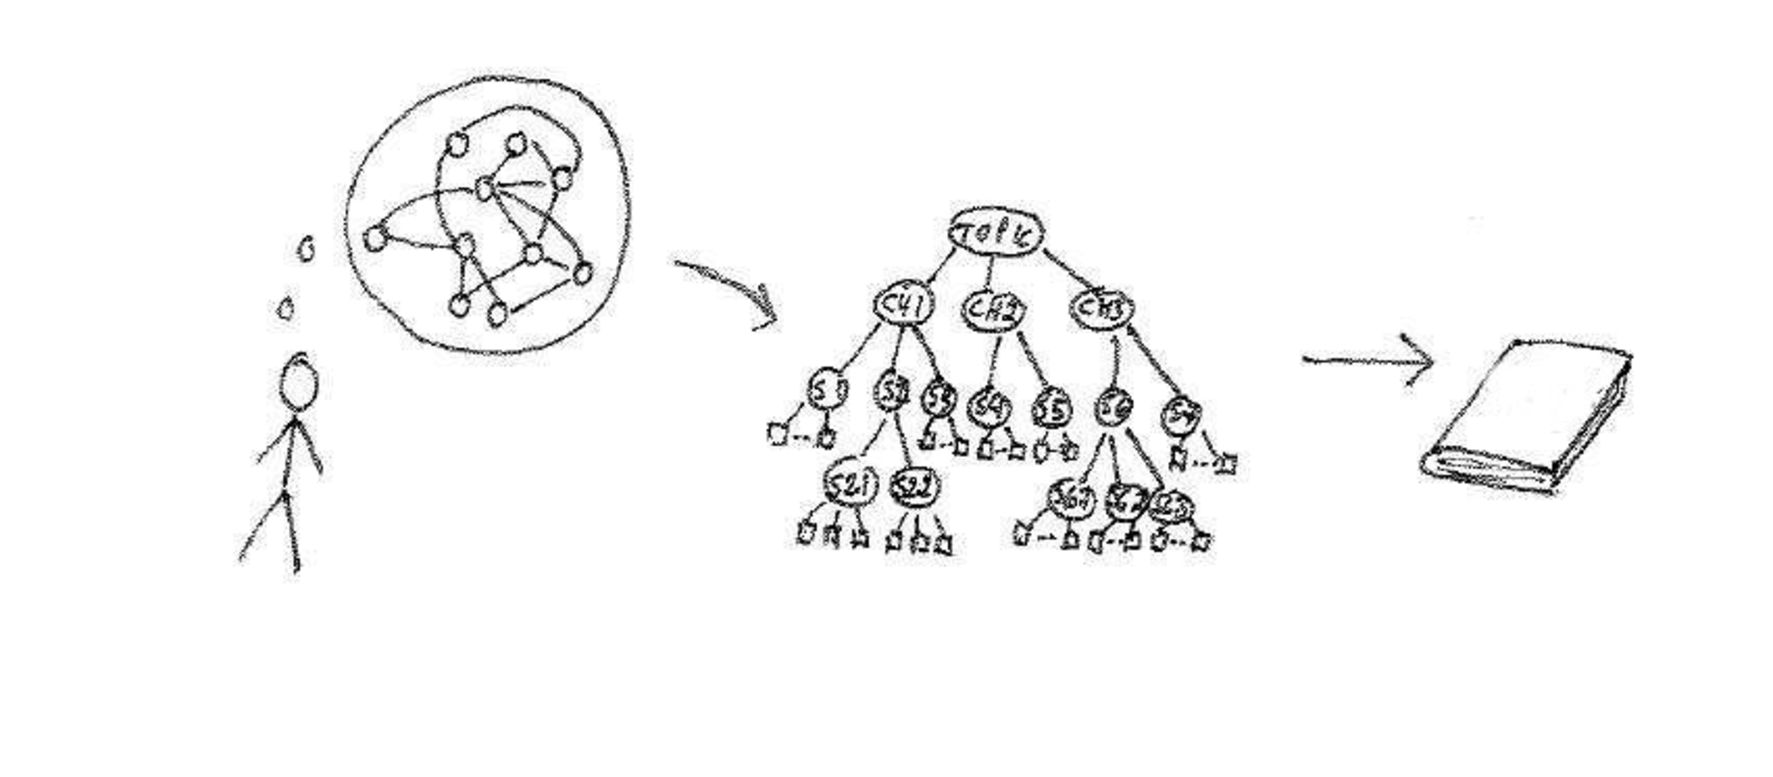
\includegraphics[width=\textwidth]{immagini/ideas2text.pdf}
\caption{Frontend di configurazione della sonda \texttt{aws\_cloudtrail} su MoonCloud.}
\label{fig:awscloudtrailform}
\end{figure}
\end{center}

L'\textit{Abstract Evaluation Rule} invece è necessaria per presentare la sonda sulla dashboard di MoonCloud, in modo che l'utente possa vederla se marcata come pubblica, identificarla anche grazie ad un'immagine di copertina, filtrarla per categoria. 

\subsection{Dashboard}
\label{sec:dashboard}

La dashboard di MoonCloud è accessibile via Web e consente di creare il proprio spazio operativo in cui definire \textit{Zone} da analizzare, quali sonde eseguire e su quali \textit{Target}, con quali credenziali eseguire le sonde e con quali parametri di configurazione.

Un account può creare più zone per suddividere le risorse da analizzare, ad esempio in base all'infrastruttura cloud pubblica, come nel caso di AWS, o in base all'infrastruttura privata come in caso di repository GitLab privati, oppure piattaforme di container come Kubernetes o Docker.  

In ogni zona è possibile creare dei \textit{Target}, ovvero le risorse da analizzare definite da un URL e a cui è possibile associare diversi tipi di credenziali, da specificare nel backend durante la creazione del controllo: tutte le sonde si basano sulla coppia \texttt{Username-Password} che per il caso specifico di AWS è \textit{Access Key ID} e \textit{Secret Access Key}; altre tipologie di credenziali sono \texttt{Git Login}, \texttt{SSH Key}. 

Una volta definito il target, nella sezione \textit{Evaluations} è possibile creare un \textit{Evaluation}, ovvero eseguire una sonda che che produce un risultato, una valutazione, che può essere positiva o negativa. Durante la creazione si seleziona la sonda di interesse, si associa ad un Target, si specificano i parametri di configurazione definiti nel form specifico della sonda ed essa viene eseguita. Inoltre, è possibile specificare se si tratta di un esecuzione \textit{One Shot} o \textit{Scheduled}, ovvero se si desidera eseguire la sonda una sola volta o se si desidera pianificarne l'esecuzione periodica ogni ora o ogni giorno.

Quando viene eseguita il risultato JSON mostrato nella sezione \ref{sec:implementazione} viene mostrato in frontend tramite un menù a tendina che consente di espandere i risultati \texttt{raw} e visualizzare le informazioni di dettaglio, come mostrato in Figura \ref{fig:awscloudtrailresult}.

\begin{center}
\begin{figure}
\centering
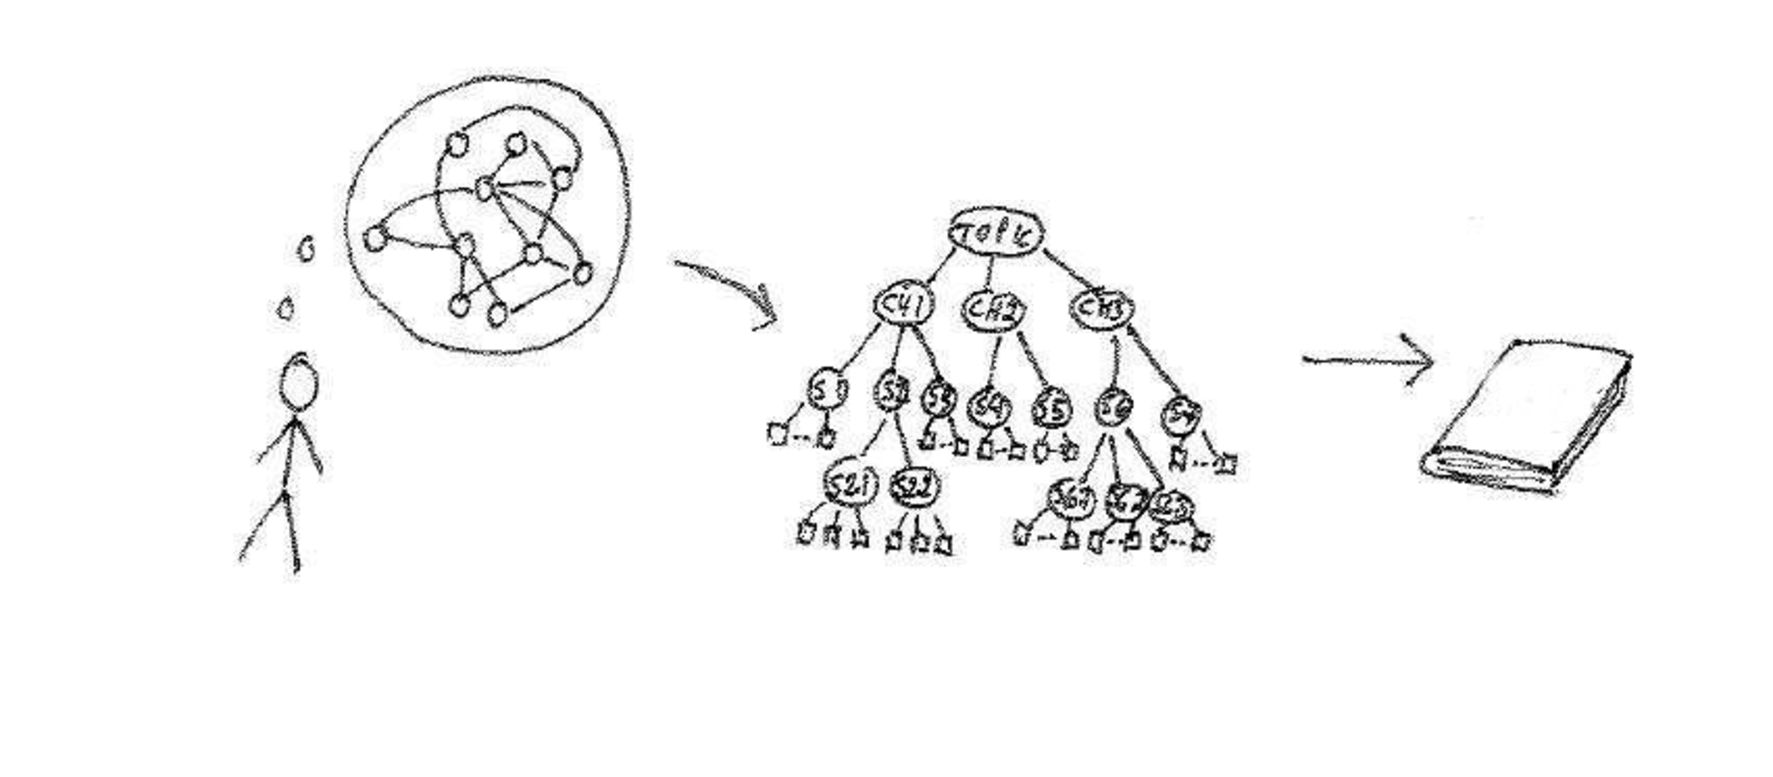
\includegraphics[width=\textwidth]{immagini/ideas2text.pdf}
\caption{Frontend di visualizzazione dei risultati della sonda \texttt{aws\_cloudtrail} su MoonCloud.}
\label{fig:awscloudtrailresult}
\end{figure}
\end{center}

Per quanto riguarda i risultati \texttt{refined} invece, essi oltre alla visualizzazione mostrata sopra hanno una sezione dedicata nel menù della dashboard, in cui è possibile ogni CVE e visualizzare informazioni come il nome, la descrizione, il punteggio CVSS per cui è possibile anche l'ordinamento, e il nome del controllo che l'ha generata: 

\begin{center}
\begin{figure}
\centering
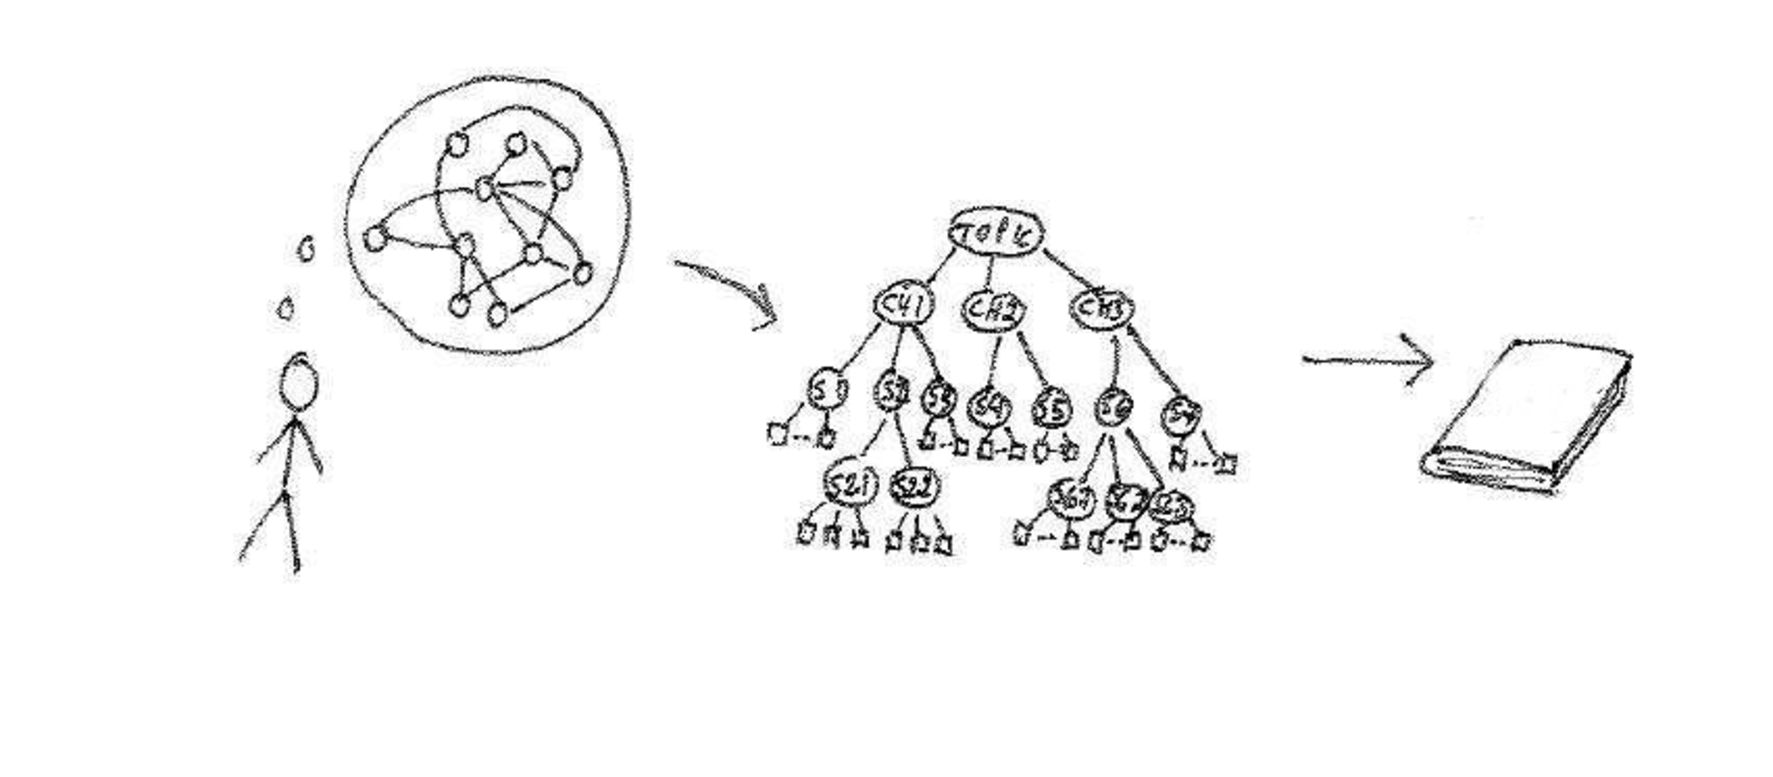
\includegraphics[width=\textwidth]{immagini/ideas2text.pdf}
\caption{Visualizzazione delle CVE su MoonCloud.}
\label{fig:mooncloudcve}
\end{figure}
\end{center}

Da ultimo, pagina principale mostra dei grafici a torta che mostrano la percentuale di compliance dell'account e di ogni zona, facendo il rapporto tra i controlli passati e quelli falliti, riportando anche la percentuale numerica. In aggiunta sono disposte al di sotto una parte delle sonde eseguite e il loro stato dopo l'ultima esecuzione.

\begin{center}
\begin{figure}
\centering
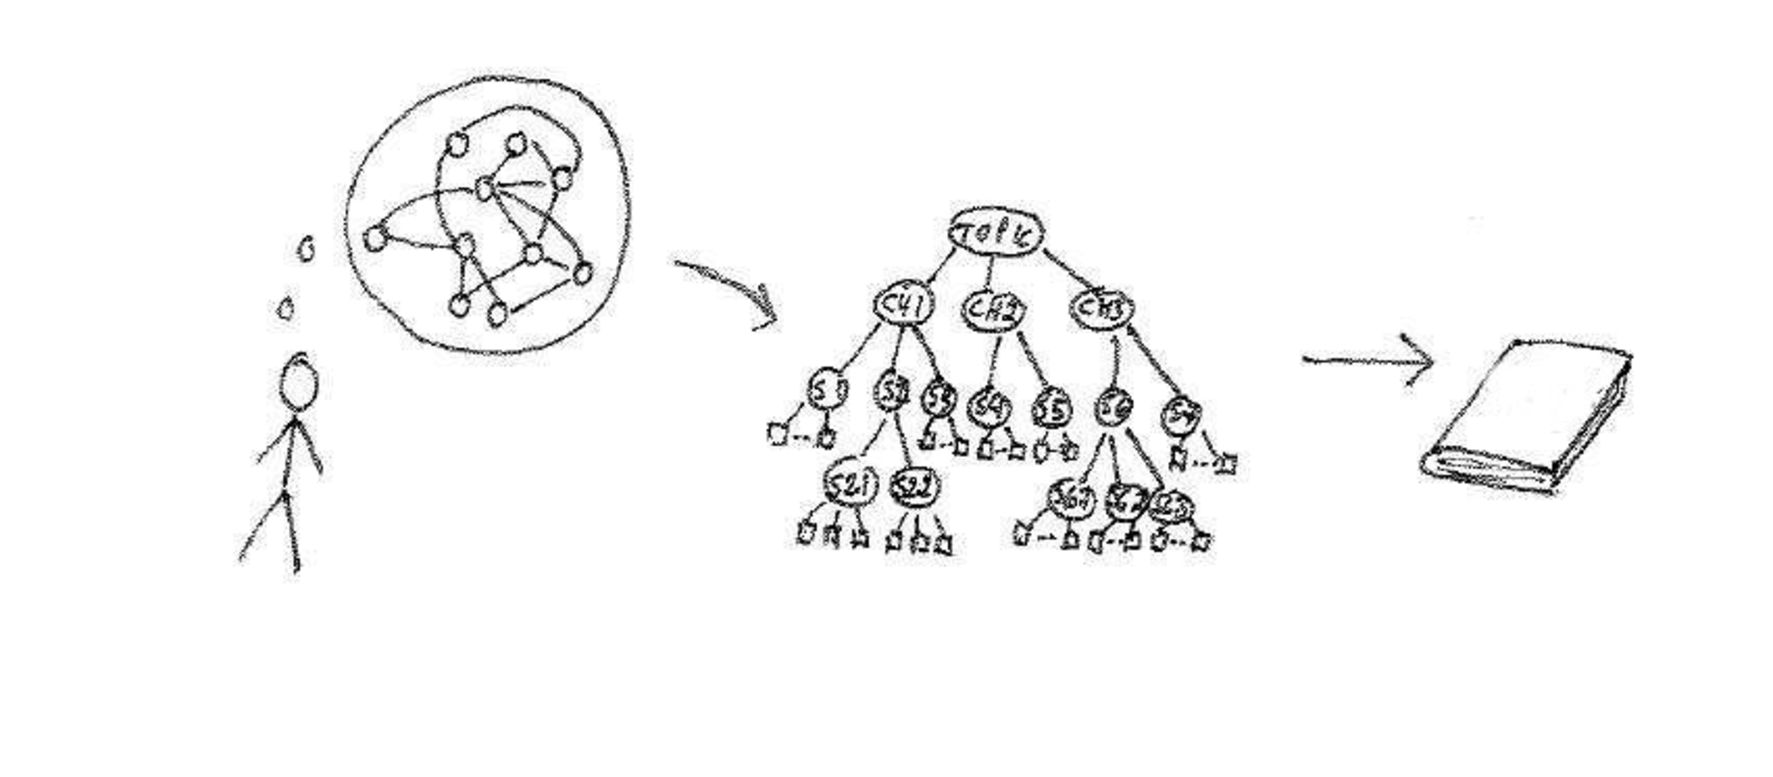
\includegraphics[width=\textwidth]{immagini/ideas2text.pdf}
\caption{Dashboard di MoonCloud con i grafici di compliance e le sonde eseguite.}
\label{fig:dashboardmooncloud}
\end{figure}
\end{center}

La dashboard di MoonCloud è l'interfaccia principale del sistema, che consente di gestire le sonde, i target e le valutazioni, e di visualizzare i risultati delle sonde eseguite. Grazie all'interfaccia intuitiva e alle funzionalità di filtraggio e ordinamento, gli utenti possono facilmente navigare tra le sonde, i target e le valutazioni, e ottenere una visione chiara dello stato di compliance delle proprie risorse cloud. 

\section{Demonstration}
\label{sec:demonstration}

Per dimostrare l'esecuzione delle sonde e la loro integrazione in MoonCloud, esse sono state eseguite su un account AWS di test, in cui sono presenti 3 Zone:

\begin{itemize}
    \item \textbf{IaaS}: zona dedicata alle infrastrutture come  
    \item \textbf{PaaS}: zona dedicata alle piattaforme come
    \item \textbf{SaaS}: zona dedicata ai servizi come 
\end{itemize}

Le sonde sono state catalogate in base alla loro tipologia e sono state eseguite su ogni zona, in modo da verificare la loro funzionalità e l'integrazione con MoonCloud.

Questo esempio dimostra come le sonde siano in grado di analizzare le risorse AWS in un contesto reale, assimilabile ad un ambiente di produzione aziendale, e come MoonCloud sia in grado di presentare in maniera chiara e intuitiva i risultati delle sonde eseguite, consentendo agli utenti di monitorare la compliance delle proprie risorse cloud in modo efficace.
    
    \chapter{Conclusioni}
\label{cap:conclusioni}

In questo capitolo si riassumono i risultati ottenuti e si discutono le implicazioni del lavoro svolto. Si evidenziano i principali aspetti del progetto, le sfide affrontate e le soluzioni implementate.

L'obiettivo di questo lavoro è stato quello di sviluppare delle soluzioni per la verifica della compliance in ambienti Cloud, in particolare AWS. La prima parte del progetto ha previsto l'analisi delle direttive CIS e NIST. Queste erano disponibili direttamente nella documentazione web di AWS Security Hub, da cui è stato semplice estrarre le richieste di ogni controllo. Per quanto riguarda invece documenti più specifici, come il CIS Amazon Elastic Kubernetes Service Benchmark, è stata necessaria la consultazione dell'intero documento per individuare i controlli pertinenti.

La scelta dei controlli da implementare è stata fatta in modo da aderire completamente alle direttive del CIS AWS Foundations Benchmark, includendo anche direttive NIST SP 800-53 per sonde riguardanti servizi come SQS, Inspector ed EKS, non trattate nel CIS.

Una volta compresi i requisiti, si è proceduto con lo studio approfondito del funzionamento della piattaforma MoonCloud e del suo driver per la realizzazione delle sonde. Questa fase ha rappresentato una delle principali sfide del progetto, poiché la comprensione della struttura delle sonde e dei parametri richiesti per l'esecuzione dei controlli è risultata fondamentale per garantirne l'integrazione corretta nella piattaforma. La programmazione delle sonde è stata effettuata in Python, utilizzando la libreria Boto3 per interagire con i servizi AWS. Anche in questo caso, la consultazione approfondita della documentazione dei client Boto3 si è rivelata cruciale per comprendere quali funzioni restituissero i parametri utili ai fini del controllo.

Una volta implementate le sonde, si è proceduto con la loro integrazione nella piattaforma MoonCloud, a partire dalla creazione nel backend di Control e Abstract Evaluation Rule. Questi sono necessari per creare una sonda eseguibile, associarvi l'immagine Docker costruita dalla pipeline CI/CD, creare un form per i parametri di input e catalogare la sonda nella dashboard di MoonCloud. 

L'ultimo passaggio ha previsto l'esecuzione delle sonde e la verifica dei risultati ottenuti sull'account di demo. I risultati sono stati soddisfacenti, dimostrando che le sonde sono in grado di verificare la compliance dei servizi AWS rispetto ai controlli implementati. Le sonde hanno prodotto output coerenti con le aspettative e le istanze di AWS sono state correttamente valutate in base ai criteri stabiliti.

Le principali sfide affrontate sono state dunque la varietà delle API tra i diversi servizi AWS e la necessità di standardizzare input e output delle sonde per consentirne l'integrazione nella dashboard di MoonCloud. Le soluzioni implementate hanno portato allo sviluppo di un sistema modulare, flessibile e capace di essere eseguito in modo automatizzato su diversi target AWS.

\section{Sviluppi futuri}
\label{sec:sviluppi_futuri}

Tra i possibili sviluppi futuri del progetto si individuano due principali direzioni:

\begin{itemize}
  \item \textbf{Estensione dell'implementazione multiregione}: attualmente solo la sonda \texttt{aws\_sqs} supporta la verifica in più regioni AWS. L'obiettivo è estendere questa funzionalità a tutte le sonde, in modo da garantire una copertura completa e centralizzata delle verifiche di compliance in scenari distribuiti su più regioni. 

  \item \textbf{Adattamento ad altri cloud provider}: la struttura modulare delle sonde e l'architettura della piattaforma MoonCloud costituiscono una buona base per estendere le verifiche di compliance anche ad altri ambienti cloud, come Microsoft Azure o Google Cloud Platform. Naturalmente, ciò richiederà modifiche alle sonde per adattarle alle API e ai servizi specifici di ciascun provider. Questo permetterebbe di ampliare l'utilizzo della piattaforma MoonCloud e di offrire un sistema di compliance più ampio e versatile.
\end{itemize}

In conclusione, il progetto ha raggiunto gli obiettivi prefissati, dimostrando la fattibilità di implementare un sistema di verifica della compliance in ambienti cloud mediante l'utilizzo di MoonCloud. I risultati ottenuti offrono una base solida per ulteriori sviluppi, contribuendo a rendere la sicurezza e la compliance nel cloud più accessibili e gestibili, anche in contesti aziendali dove si desidera una supervisione continua e automatizzata della sicurezza in questo ambito.

    
    
    \appendix
    \chapter{aws\_sqs}
    \label{app:sqs}
    \lstinputlisting[style=mypython]{code/sqs.py}
    
    \chapter{aws\_inspector}
    \label{app:inspector}
    \lstinputlisting[style=mypython]{code/inspector.py}

    \chapter{aws\_vulnerability}
    \label{app:aws_vulnerability}
    \lstinputlisting[style=mypython]{code/vuln.py}
    
    %
    %			BIBLIOGRAFIA
    %
    
    % Si può specificare a che livello della TOC deve essere la bibliografia.
    % Il default è 'chapter', per 'part' usare
    % \beforebibliography[part]
    \beforebibliography
    \bibliographystyle{unsrt}
    \bibliography{bibliografia}
    
    % Pagina di chiusura
    \closingpage
    
    \end{document}